\documentclass[12pt]{article}

% Load packages
\usepackage{url}  % Formatting web addresses
\usepackage{ifthen}  % Conditional
\usepackage{multicol}   %Columns
\usepackage[utf8]{inputenc} %unicode support
\usepackage{amsmath}
\usepackage{amssymb}
\usepackage{epsfig}
\usepackage{epstopdf}
\usepackage{graphicx}
\usepackage{cite}
\usepackage{lastpage,fancyhdr,graphicx}
\usepackage{mathtools}
\usepackage[margin=0.1pt,font=footnotesize,labelfont=bf]{caption}
\usepackage{setspace}
%\usepackage{longtable}
\usepackage{colortbl}
%\usepackage{palatino,lettrine}
%\usepackage{times}
%\usepackage[applemac]{inputenc} %applemac support if unicode package fails
%\usepackage[latin1]{inputenc} %UNIX support if unicode package fails
\usepackage[wide]{sidecap}
%\usepackage[authoryear,round,comma,sort&compress]{natbib}
\usepackage[square,sort,comma,numbers,sort&compress]{natbib}
%\usepackage[authoryear,round]{natbib}
\usepackage{supertabular}
\usepackage{simplemargins}
\usepackage{fullpage}
\usepackage{comment}
\usepackage{lineno}
%\usepackage{chicago}
\usepackage{textcomp}
\usepackage{multirow}
\usepackage{amsmath}
%\usepackage{textgreek}
%\usepackage[linesnumbered,lined,boxed,commentsnumbered]{algorithm2e}
\DeclareMathOperator*{\argmin}{\arg\!\min}

%\usepackage{algorithm2e}
%\usepackage{algpseudocode}
%\usepackage[space]{cite}
\urlstyle{rm}
\hyphenation{dec-ades} %Latex does not know how to hyphenate this by default, so we add it to the list

%\textwidth = 6.50 in
%\textheight = 9.5 in
%\oddsidemargin =  0.0 in
%\evensidemargin = 0.0 in
%\topmargin = -0.50 in
%\headheight = 0.0 in
%\headsep = 0.25 in
%\parskip = 0.15in
%\linespread{1.75}
\doublespace

%\bibliographystyle{chicago}
\bibliographystyle{plos2009}

\makeatletter
\renewcommand\subsection{\@startsection
	{subsection}{2}{0mm}
	{-0.05in}
	{-0.5\baselineskip}
	{\normalfont\normalsize\bfseries}}
\renewcommand\subsubsection{\@startsection
	{subsubsection}{2}{0mm}
	{-0.05in}
	{-0.5\baselineskip}
	{\normalfont\normalsize\itshape}}
\renewcommand\section{\@startsection
	{subsection}{2}{0mm}
	{-0.2in}
	{0.05\baselineskip}
	{\normalfont\large\bfseries}}
\renewcommand\paragraph{\@startsection
	{paragraph}{2}{0mm}
	{-0.05in}
	{-0.5\baselineskip}
	{\normalfont\normalsize\itshape}}
\makeatother

%Review style settings
%\newenvironment{bmcformat}{\begin{raggedright}\baselineskip20pt\sloppy\setboolean{publ}{false}}{\end{raggedright}\baselineskip20pt\sloppy}

%Publication style settings

% Single space'd bib -
\setlength\bibsep{0pt}

\renewcommand{\rmdefault}{phv}\renewcommand{\sfdefault}{phv}
\newcommand{\norm}[1]{\left\lVert#1\right\rVert}

% Change the number format in the ref list -
\renewcommand{\bibnumfmt}[1]{#1.}

% Change Figure to Fig.
\renewcommand{\figurename}{Fig.}

% Begin ...
\begin{document}
\begin{titlepage}
{\par\centering\textbf{\Large {Toward a Genome Scale Dynamic Model of Cell-Free Protein Synthesis in \emph{Escherichia~coli}}}}
\vspace{0.05in}
{\par \centering \large{Nicholas Horvath, Michael Vilkhovoy, Joseph Wayman, Kara Calhoun$^{1}$, James Swartz$^{1}$ and Jeffrey D. Varner$^{*}$}}
\vspace{0.10in}
{\par \centering {Robert Frederick Smith School of Chemical and Biomolecular Engineering}}
{\par \centering {Cornell University, Ithaca NY 14853}}
\vspace{0.1in}
{\par \centering {$^{1}$School of Chemical Engineering}}
{\par \centering {Stanford University, Stanford, CA 94305}}
{\par \centering \textbf{Running Title:}~Dynamic modeling of cell-free protein synthesis}
\vspace{0.1in}
{\par \centering \textbf{To be submitted:}~\emph{Scientific~Reports}}
\vspace{0.5in}
{\par \centering $^{*}$Corresponding author:}
{\par \centering Jeffrey D. Varner,}
{\par \centering Professor, Robert Frederick Smith School of Chemical and Biomolecular Engineering,}
{\par \centering 244 Olin Hall, Cornell University, Ithaca NY, 14853}
{\par \centering Email: jdv27@cornell.edu}
{\par \centering Phone: (607) 255 - 4258}
{\par \centering Fax: (607) 255 - 9166}
\end{titlepage}
\date{}
\thispagestyle{empty}
\pagebreak
%%%%%%%%%%%%%%%%%%%%%%%%%%%%%%%%%%%%%%%%%%%%%%%%%%%%%%%%%%%%%%%%%%%%%%%%%%%%%%%%%%%%%%%%%%%%%%%%%%%%%%%%%%%
%%%%%%%%%%%%%%%%%%%%%%%%%%%%%%%%%%%%%%%%%%%%%%%%%%%%%%%%%%%%%%%%%%%%%%%%%%%%%%%%%%%%%%%%%%%%%%%%%%%%%%%%%%%
\section*{Abstract}
Cell-free protein expression systems have become widely used in systems and synthetic biology.
In this study, we developed an ensemble of dynamic \textit{E. coli} cell-free protein synthesis (CFPS) models.
Model parameters were estimated from measurements of glucose, organic acids, energy species, amino acids, and the protein product, chloramphenicol acetyltransferase (CAT).
The ensemble described all of the training data, especially the central carbon metabolism.
The model predicted a carbon yield for CAT production that was equal to 23\% of the maximum theoretical yield, calculated using sequence-specific flux balance analysis.
This suggests that CAT production could be further optimized.
The dynamic modeling approach predicted that substrate consumption of glucose and pyruvate and oxidative phosphorylation were most important to both CAT production and the system as a whole, while CAT production alone depended heavily on the CAT synthesis reaction.
Conversely, CAT production was robust to allosteric control, as was most of the network, with the exception of the organic acids in central carbon metabolism.
This study is the first to model dynamic protein production in \textit{E. coli}, and should provide a foundation for genome-scale,
dynamic modeling of cell-free \textit{E. coli} protein synthesis.

\vspace{0.1in}
{\noindent \textbf{Keywords:}~Biochemical engineering, systems biology, cell-free protein synthesis}

\pagebreak

\setcounter{page}{1}

%In this study, we present a framework for dynamic, cell-free metabolic modeling, integrating a simple logical description of regulation with traditional enzyme kinetics.
%Using this framework, we have constructed an ensemble of models for production of chloramphenicol acetyltransferase in a cell-free \textit{E. coli} system.
%Our ensemble fits measurements of glucose, chloramphenicol acetyltransferase, organic acids, and energy species, but fails to capture much of the amino acid dynamics in the dataset.

% Uncomment in production -
\linenumbers


% Interestingly, many of the challenges confronting genome-scale kinetic modeling can potentially be overcome in a cell-free system.
% For example, there is no complex transcriptional regulation to consider, transient metabolic measurements are easier to obtain, and we no longer have to consider cell growth.
% Thus, cell-free operation holds several significant advantages for model development, identification and validation. Theoretically, genome-scale cell-free kinetic models may be possible for industrially important organisms,
% such as \textit{E. coli} or \textit{B.~subtilis}, if a simple, tractable framework for integrating allosteric regulation with enzyme kinetics can be formulated.
% Conversely, highly abstracted kinetic frameworks, such as the cybernetic framework, represented a paradigm shift, viewing cells as growth-optimizing strategists \citep{1985_dhurjati_ramkrishna_tsao_BiotechBioeng}.
% Cybernetic models have been highly successful at predicting metabolic choice behavior, e.g., diauxie behavior \citep{1986_kompala_ramkrishna_tsao_BiotechBioeng}, steady-state multiplicity \citep{2012_kim_ramkrishna_BiotechProg}, as well as the cellular response to metabolic engineering modifications \citep{1999_varner_ramkrishna_MetaEng}.
% Unfortunately, traditional, fully structured cybernetic models also suffer from an identifiability challenge, as both the kinetic parameters and an abstracted model of cellular objectives must be estimated simultaneously.
% However, recent cybernetic formulations from Ramkrishna and colleagues have successfully treated this identifiability challenge through elementary mode reduction~\cite{2009_song_ramkrishna_BiotechBioeng,Song:2011aa}.

\section*{Introduction}

Cell-free systems offer many advantages for the study, manipulation and modeling of metabolism compared to \textit{in vivo} processes.
Central amongst these, is direct access to metabolites and the biosynthetic machinery without the interference of a cell wall, or complications associated with cell growth.
This allows us to interrogate the chemical environment while the biosynthetic machinery is operating, potentially at a fine time resolution.
Cell-free protein synthesis (CFPS) systems are arguably the most prominent examples of cell-free systems used today \citep{Jewett:2008aa}.
However, CFPS is not new; CFPS in crude \textit{E.~coli} extracts has been used since the 1960s to explore fundamentally important biological mechanisms \citep{MATTHAEI:1961aa,NIRENBERG:1961aa}.
Today, cell-free systems are used in a variety of applications ranging from therapeutic protein production \citep{Lu:2014aa} to synthetic biology \citep{Hodgman:2012aa,Pardee:2016aa}.
However, if CFPS is to become a mainstream technology for applications such as point of care manufacturing, we must first understand the performance limits of these systems.
One tool to address this question is mathematical modeling.

Mathematical modeling has long contributed to our understanding of metabolism.
Decades before the genomics revolution, mechanistically structured metabolic models arose from the desire to predict microbial phenotypes resulting from changes in intracellular or extracellular states \citep{1976_fredrickson_BiotechBioeng}.
The single cell \textit{E. coli} models of Shuler and coworkers pioneered the construction of large-scale, dynamic metabolic models that incorporated multiple, regulated catabolic and anabolic pathways constrained by experimentally determined kinetic parameters \citep{1984_domach_shuler_BiotechBioeng_01}.
Shuler and coworkers generated many single cell kinetic models, including single cell models of eukaryotes \citep{1989_steinmeyer_shuler_ChemEngSci,1992_wu_shuler_AnnNYAcadSci}, minimal cell architectures \citep{2004_castellanos_shuler_PNAS}, as well as DNA sequence based whole-cell models of \textit{E. coli} \citep{2008_atlas_shuler_IETSysBio}.
In the post genomics world, large-scale stoichiometric reconstructions of microbial metabolism popularized by techniques such as flux balance analysis (FBA) have become a standard approach \citep{2012_lewis_palsson_NatRevMicrobio}.
Since the first genome-scale stoichiometric model of \textit{E. coli}, developed by Edwards and Palsson \citep{2000_edwards_palsson_PNAS}, well over 100 organisms, including industrially important prokaryotes are now available \citep{2009_feist_palsson_NatRevMicrobio,Feist:2007aa,Oh:2007aa}.
Stoichiometric models rely on a pseudo-steady-state assumption to reduce unidentifiable genome-scale kinetic models to an underdetermined linear algebraic system, which can be solved efficiently even for large systems.
Traditionally, stoichiometric models have also neglected explicit descriptions of metabolic regulation and control mechanisms, instead opting to describe the choice of pathways by prescribing an objective function on metabolism. Interestingly, similar to early cybernetic models, the most common metabolic objective function has been the optimization of biomass formation \citep{2002_ibarra_edwards_palsson_Nat}, although other metabolic objectives have also been estimated \citep{2007_schuetz_sauer_MolSysBio}.
Recent advances in constraint-based modeling have overcome the early shortcomings of the platform, including capturing metabolic regulation and control \citep{2013_hyduke_lewis_palsson_MolBioSys}.
Thus, modern constraint-based approaches have proven extremely useful in the discovery of metabolic engineering strategies and represent the state of the art in metabolic modeling \citep{2013_mccloskey_palsson_feist_MolSysBio, 2012_zomorrodi_maranas_MetaEng}.
However, genome-scale kinetic models of industrial important organisms such as \textit{E. coli} have yet to be constructed.

In this study, we developed an ensemble of kinetic cell-free protein synthesis (CFPS) models using dynamic metabolite measurements in an \textit{E. coli} cell free extract.
Model parameters were estimated from measurements of glucose, organic acids, energy species, amino acids, and the protein product, chloramphenicol acetyltransferase (CAT).
Characteristic values for model parameters and initial conditions, estimated from literature, were used to constrain the parameter estimation problem.
The ensemble of parameter sets described the training data with a median cost that was greater than two orders of magnitude smaller than random sets constructed using the literature parameter constraints. We then used the ensemble of kinetic models to analyze the CFPS reaction.
First, sensitivity analysis of the dynamic model suggested that CAT production was most sensitive to CAT synthesis parameters, as well as reactions in oxidative phosphorylation and pyruvate consumption.
Sensitivity analysis also showed that the system as a whole was most sensitive to these same parts of the network and glucose consumption.
CAT production and other metabolites, specifically organic acid intermediates such as pyruvate, were sensitive to the presence of allosteric control mechanisms.
Next, to gauge the performance of the cell-free reaction, we compared the observed CAT carbon yield with the maximum theoretical CAT carbon yield calculated using sequence-specific flux balance analysis. The CAT yield estimated from the kinetic model was 23\% of the maximum theoretical yield, but 36\% of the theoretical yield when physiologically realistic constraints were used. 
Taken together, we have integrated traditional kinetics with a logical rule-based description of allosteric control to simulate a comprehensive CFPS dataset.
This study provides a foundation for genome-scale, dynamic modeling of cell-free \textit{E. coli} protein synthesis.

% In this study, we present an effective biochemical network modeling framework for building dynamic cell-free metabolic models.
% The key innovation of our approach is the seamless integration of simple effective rules encoding complex regulation with traditional kinetic pathway modeling.
% This integration allows the description of complex regulatory interactions in the absence of specific mechanistic information.
% The regulatory rules are easy to understand, easy to formulate and do not rely on overarching theoretical abstractions or restrictive assumptions.
% Using this approach, we have built an ensemble of models that predict an experimental dataset for CAT production in a cell-free \textit{E. coli} system.
% We calculated the CAT yield for the ensemble at 45\% of the theoretical maximum according to constraint-based modeling, and determined through sensitivity analysis that CAT production was most sensitive to the parameters associated with CAT synthesis and the synthesis of GTP, GMP, and amino acids.
% While only an initial proof-of-concept, the framework presented here could be an important first step toward genome-scale cell-free kinetic modeling of the biosynthetic capacity of industrially important organisms.

\clearpage

\section*{Results}

The ensemble of kinetic CFPS models captured the time evolution of CAT biosynthesis (Fig.~\ref{fig:CarbonBoth} - \ref{fig:Amino}).
The cell-free \textit{E.~coli} metabolic network was constructed by removing growth associated reactions from the iAF1260 reconstruction \cite{Feist:2007aa},
and by adding reactions describing chloramphenicol acetyltransferase (CAT) biosynthesis, a model protein for which we have a comprehensive training dataset \cite{2005_calhoun_BiotechnologyProgress}.
The CFPS model equations were formulated using the hybrid cell-free modeling framework of Wayman et al. \cite{pr3010138}.
An ensemble of model parameters (N $>$ 10,000) was estimated from measurements of glucose, CAT, organic acids (pyruvate, lactate, acetate, succinate, malate), energy species (A(x)P, G(x)P, C(x)P, U(x)P), and 18 of the 20 proteinogenic amino acids using a constrained Markov Chain Monte Carlo (MCMC) approach.
The MCMC algorithm minimized the error between the training data and model simulations starting from an initial parameter set assembled from literature and inspection.
Parameter sets were selected for the ensemble based upon their error, and the Pearson correlation coefficient between the candidate and existing sets in the ensemble.
The parameter set with the lowest error value was defined as the best-fit set.
Central carbon metabolism (Fig.~\ref{fig:CarbonBoth}, top), energy species (Fig.~\ref{fig:Energy}), and amino acids (Fig.~\ref{fig:Amino}) were captured by the ensemble and the best-fit set.
The constrained MCMC approach estimated parameter sets with a median error greater than two-order of magnitude less than random parameter sets generated within
the same parameter bounds (Fig. \ref{fig:BoxPlot}); thus, we have confidence in the predictive capability of the estimated parameters.
Allosteric control was important to the dynamics of the organic acid intermediates and CAT biosynthesis (Fig.~\ref{fig:CarbonBoth}, bottom).
The acetate, lactate, pyruvate, succinate, malate and CAT trajectories were qualitatively different in the absence of allosteric control following glucose exhaustion.
In particular, the rate of CAT biosynthesis and lactate accumulation and subsequent consumption decreased following glucose exhaustion in the absence of control.

% We used the hybrid cell-free modeling framework of Wayman and coworkers to simulate the production of CAT \citep{pr3010138}.
% The cell-free \textit{E. coli} metabolic network was constructed by removing the growth-associated processes from the model of Palsson and coworkers \cite{2000_edwards_palsson_PNAS}, and by adding reactions for the synthesis of
% Thus, the model described core central carbon metabolism (glycolysis, pentose phosphate, Enter-Doudoroff, TCA cycle), as well as the synthesis of energy species, amino acids biosynthesis and degradation, and biosynthesis of the CAT protein.
% An ensemble of model parameters was estimated from dynamic measurements of glucose, CAT, organic acids (pyruvate, lactate, acetate, succinate, malate), energy species (A(x)P, G(x)P, C(x)P, U(x)P), and 18 of the 20 proteinogenic amino acids by minimizing the difference between the experimental dataset and metabolite simulations subject to literature constraints on parameter values and initial conditions.
% We performed a local sensitivity analysis to determine the network reactions with the greatest effect on protein production and overall system state.

To better understand which parameters and parameter combinations influenced model performance we performed sensitivity analysis (Fig.~\ref{fig:Sensitivity}).
CAT production was most sensitive to the CAT synthesis reaction, oxidative phosphorylation activity, and alanine synthesis (Fig.~\ref{fig:Sensitivity}, top, section A).
The 16 next most important reactions to CAT production (section B) came from various pathways across the network: four each from glycolysis, the TCA cycle, and amino acid synthesis/degradation; two from the pentose phosphate pathway; and one each from the Entner-Doudoroff pathway and the energy species reactions.
The pairwise sensitivities (off-diagonal elements) were different from the corresponding first-order sensitivities (diagonal elements), and led to interesting outcomes.
For example, glutamine synthesis and arginine degradation were both among the most important reactions to CAT production (they rank 5th and 10th, respectively).
This was likely because they both affect the sensitive glutamine-glutamate balance; glutamine synthesis consumes glutamate, while arginine degradation produces it.
However, when both were perturbed, their combined effect on the model was low, as the respective contributions to consumption and production of glutamate cancelled.
The system state as a whole was most sensitive to glucose uptake via GTP and the forward reaction of lactate dehydrogenase (Fig.~\ref{fig:Sensitivity}, bottom, section F).
The 30 next most important reactions to the system state (section G) came from various pathways across the network: eight from amino acid synthesis/degradation; six from glycolysis; four from the TCA cycle; and two each from the pentose phosphate pathway, Entner-Doudoroff, energy/reducing pathways, and small molecule transport; one from oxidative phosphorylation; and one from pyrophosphatase consumption. The system state had more pairwise sensitivities that differ from the corresponding first-order sensitivities and stand out as significant.
For example, the first-order effect of alanine synthesis was large; it consumes both pyruvate and glutamate, two key species in the network.
In addition, a handful of alanine synthesis pairwise sensitivities were also large.
However, there were enough reactions that, when paired with alanine synthesis, had little effect on the model; malic enzyme is one of these, as it produces the pyruvate that alanine synthesis consumes. Thus, the total-order alanine synthesis sensitivity was low, placing it at the very bottom of section I.
Another interesting result was the intersection of sections F and G with section J.
The 53 reactions in section J were turned off in the best-fit set (rate constants were set to 0);
therefore, the perturbation of these reactions had no effect on the model.
Thus, all pairwise sensitivities with reactions in section J were pseudo first-order sensitivities for the other reactions.
Interestingly, many reactions in section F and several in section G showed their highest sensitivities when paired with the "non-effects" of section J.
Of these, three involved pyruvate, strengthening its role as a key metabolite; the others were glucose consumption via GTP/CTP-specific hexokinases,
fumarate reductase, and SO$_4$ utilization.
This suggested that these reactions' effects on the model were canceled out or lessened by most other reactions, but were of course not affected by the reactions in section J.
This was also likely the reason that reactions in section J rank above those in section K, despite having no effect themselves on the model.
Taken together, sensitivity analysis identified blocks of parameters that either individually, or in combination influenced model performance.
However, the sensitivity analysis did not establish what the maximum performance of the system was.
To answer that question we performed sequence-specific flux balance analysis of CAT production.

We used sequence-specific flux balance analysis (ssFBA) to calculate the theoretical maximum CAT carbon yield for different constraint values (Fig.~\ref{fig:CATProdYield}).
The experimental CAT carbon yield was 0.0821, while the best-fit parameter set had a carbon yield of 0.086 $\pm$ 0.004.
Thus, although the kinetic model described the experimental data including the yield, it was unclear whether the performance of the CFPS system was optimal.
To address this question, we used ssFBA in combination with the cell-free metabolic network and a T7 promoter model to estimate the maximum theoretical CAT carbon yield.
Toward this, we first validated the ssFBA approach by comparing the simulated versus measured concentrations of CAT over the first hour of the CFPS reaction (Fig.~\ref{fig:CATProdYield}A).
We sampled different RNA polymerase/ribosome levels and elongation rates in the physiological range to establish the uncertainty in the ssFBA simulation.
The ssFBA estimate of the CAT abundance was consistent with the measured values. Next, we calculate the CAT carbon yield for three classes of constraints:
(i) theoretical max glucose, amino acid and oxygen upper bounds, and no transcriptional/translational constraints; (ii) theoretical maximum glucose, amino acid and oxygen upper bounds,
and realistic transcriptional/translational constraints and (iii) metabolite values constrained by the data, and realistic transcriptional/translational constraints.
The unconstrained theoretical maximum CAT carbon yield was 0.363 $\pm$ 0.02 (Fig.~\ref{fig:CATProdYield}B, left);
this case had no upper bound on the transcription and translation reactions, and was only constrained by glucose, oxygen and amino acid consumption rates.
On the other hand, for realistic constraints on transcription and translation, the CAT carbon yield was 0.226 $\pm$ 0.03 (Fig.~\ref{fig:CATProdYield}B, middle).
Lastly, when using realistic metabolite and transcription and translation constraints the predicted carbon yield was 0.062 $\pm$ 0.02, similar to the experimental yield Fig.~\ref{fig:CATProdYield}B, end).
Thus, the experimental dataset and best-fit parameter set each produced CAT at 23\% of the theoretical maximum and 36\% of a theoretical physiological case.

In comparing the flux distributions between the unconstrained and constrained cases (Fig.~\ref{fig:Network}), the constrained cases heavily utilized the first step in the pentose phosphate pathway to generate NADPH.
In these cases the majority of the flux continued through the Entner–Doudoroff pathway, whereas in the unconstrained case the majority of flux traveled through glycolysis.
In all cases, the energy source came primarily from oxidative phosphorylation, as well as partly from the TCA cycle.
In the transcription/translation constrained case, there was a high flux through fumerate dehydrogenase from aspartic acid uptake, whereas in the unconstrained and most constrained cases, acetate and lactate accumulation occurred.
This shows that the system is producing NADH through lactate dehydrogenase as well as through pyridine nucleotide transhydrogenase (\textit{pntAB}) to supply enough NADH for oxidative phosphorylation.
As a result, high oxidative phosphorylation activity relative to our cell-free system leads to an acetate overflow.
This suggests that there is potential for increasing CAT production by reducing this diversion of carbon.
To simulate potential knockouts, we constrained the specific glucose and amino acid uptake rates to the same values as simulated with no knockouts.
In an ssFBA simulation with constrained transcription/translation rates, knocking out the \textit{gnd} reaction decreases flux of acetate production but increases flux through \textit{pntAB}, which is responsible for regenerating NADPH.
The simulation showed carbon was diverted toward lactate; however, since CAT production is constrained by the translation rate, we expected no increase in CAT production.
The decrease in acetate production is promising as a mechanism to increase CAT yield.
A second simulation with a knockout of \textit{gnd} and phosphate acetyltransferase showed carbon being diverted toward lactate and succinate; however, it required a higher flux through oxidative phosphorylation and the TCA cycle to meet the energetic needs of the system.

\clearpage

\section*{Discussion}

%The discussion has three (sometimes four) paragraphs:
%\begin{enumerate}
%	\item{\textbf{First~paragraph}: Present a modified version of the last paragraph of the introduction. In this study, [...]. Taken together, [killer statement]}
%	\item{\textbf{Second~paragraph}: Contrast the key findings of the study with other computational/experimental studies}
%	\item{\textbf{Third~paragraph}: Present future directions. If you had more time, what would like to do? Highlight the key shortcomings of the approach and how will we address them in the future.
%	In this case, we will have a scaling issue if we extend to genome scale. We should extend to dynamic cases, and we need to experimentally validate the findings.}
%\end{enumerate}

In this study we present an ensemble of \textit{E. coli} cell-free protein synthesis (CFPS) models that accurately predict a comprehensive CFPS dataset of glucose, CAT, central carbon metabolites, energy species, and amino acid measurements.
We used the hybrid cell-free modeling approach of Wayman and coworkers, which integrates traditional kinetic modeling with a logic-based description of allosteric regulation.
We showed that the model produces CAT at 23\% of the theoretical maximum in terms of carbon yield, and at 36\% of a physiological case in which transcription and translation are constrained.
The theoretical maximum and transcription/translation constrained case were obtained using FBA, which predicted a different flux distribution for each case.
The unconstrained case predicted most of the carbon flux going through glycolysis, while the constrained cases predicted significant flux through the Entner-Doudoroff pathway and some through TCA cycle.
However, all cases relied on oxidative phosphorylation for the system's energetic needs as well as for tRNA charging for CAT synthesis.
Sensitivity analysis of the dynamic model suggested that both CAT production and the entire metabolic network were most sensitive to amino acid synthesis and degradation reactions, and reactions in glycolysis and the TCA cycle.
CAT production was also very sensitive to the CAT synthesis reaction, unsurprisingly.
The allosteric control component of the hybrid modeling approach was shown as important to central carbon metabolism, but not very important to CAT production.
Taken together, this is the first dynamic model of \textit{E. coli} cell-free protein synthesis, and an important step toward a functional genome scale description.

We present an ensemble of models that quantitatively describes the system behavior of cell-free metabolism and production of CAT.
Experimental observations of the metabolites and cometabolites validate the structure of the model and the estimation of kinetic parameters. 
This is important in applying metabolic engineering principles to rationally design cell-free production processes and predict the redirection of carbon fluxes to product forming pathways.
The most sensitivite parameters for model performance are the uptake of glucose followed by pyruvate.
This outstanding control on model performace was expected as these metabolites are responsible for driving CFPS and represent the first step in the model network.
Nevertheless there are further reactions that excercise considerable sensitivity to model performance. 
Oxidative phosphorylation activity shows to be vital to model performance, since it provides most of the energetic demands of CFPS according to the model.  
In examining oxidative phosphorylation activity, knockouts in the electron transport pathways disrupt model performance and show CAT carbon yield dropping from 8.6\% to 2.7\%, consistent with literature observations\cite{2008_jewett_molsysbiol}.
Additional reactions with considerable sensitivity are responsible for the consumption of glucose and pyruvate followed by the accumulation of pyruvate which allows it to be consumed during the second phase of CFPS. 
Following these reactions, the first step in pentose phosphate pathway is important as it degrades G6P to 6PG and produces NADPH.
The interconversion of NADPH to NADH shows to be the next sensitive reaction, which helps to supply NADH to oxidative phosphorylation reactions to meet the energetic needs of the system. 
The insignificant reactions lead to the accumulation of unwanted byproducts such as ethanol and formate.

In analyzing the model sensitive parameters for CAT production, CAT synthesis followed by oxidative phosphorylation are the most sensitive.
Following these reactions, the same theme of significance is seen as in the sensitivity of overall model performace. 
The most important are glucose and pyruvate consuming reactions followed by downstream reactions from their respective products which is necessary to drive CFPS.
In addition, the conversion of ATP to GTP shows significance since it aides in the translation of CAT.
Thus to improve the efficiency of CAT production, supplementation with additional GTP may be of some benefit. 
The overall sensitivity results show the substrates driving CFPS are vital to CFPS performance and CAT production, this can be seen by the biphasic operation of CFPS. 
CFPS has biphasic formation of CAT, with the first phase operating on glucose and the second phase operating on pyruvate. 
During the first phase, there is an accumulation of metabolite byproducts from central carbon with the majority of flux going towards acetate and some towards pyruvate, lactate, and succinate but these are consumed in the second phase, except for acetate. 
CFPS operating under glucose consumption has a higher production flux of CAT than that of pyruvate/lactate consumption. 
In comparing the theoretical maximum carbon yield of CAT from ssFBA predictions to the kinetic model and experimental measurements, this suggests that there is potential for increasing CAT yield in CFPS as well as CFPS performance.
%Yield performance can be potentially improved by diverting carbon flux away from acetate. 
The theoretical maximum yield of CAT was 36\% for an unconstrained case and 22.6\% for a transcription/translation constrained case.
Knockouts of \textit{gnd} and phosphate acetyltransferase show carbon can be diverted away from acetate and potentially toward CAT or other proteins of interest expressed in CFPS.
Another limitation to be addressed in CFPS is the transcription and translation description, since the protein of interest to be expressed is ultimately bounded by these kinetic rates.
Li et al. have increased productivity of firefly lucifease by 5-fold in CFPS systems by adding and adjusting factors that affect transcription and translation such as elongation factors, ribosome recyclcing factor, release factors, chaperones, BSA, and tRNAs \cite{2014_li_PlosOne}.
Underwood and coworkers have also shown that an increase in ribosome levels does not significantly increase protein yields or rates; however, adding elongation factors increased yields by 23\% at 30 minutes \cite{2005_underwood_biotech}.
In addition to improving CFPS performance, Jewett and coworkers have shown that oxidative phosphorylation operates in cell-free systems, and that knocking out these reactions is detrimental to protein yield\cite{2008_jewett_molsysbiol}.
However, it is unknown how active oxidative phosphorylation is compared to that of \textit{in vivo} systems, and both of the modeling approaches we present suggest that oxidative phosphorylation is important to CAT production.
Thus, this is a potential area for improvement of CFPS performance and protein yield.


%The ensemble of models captured the dynamic distribution of metabolic flux.
%The ensemble of dynamic models predicted that most of the carbon flux going through glycolysis and the TCA cycle,
%while the constraint-based approach predicted most of the carbon flux went through the Entner-Doudoroff pathway and only part of glycolysis.
% We present the first dynamic, cell-free model of \textit{E. coli} metabolism and biosynthesis at this scope.
% While the early models of Shuler and coworkers achieved large-scale, dynamic descriptions of single cells \citep{1984_domach_shuler_BiotechBioeng_01}, and the stoichiometric models associated with the FBA approach are computationally efficient amd widespread \citep{2009_feist_palsson_NatRevMicrobio}, none have yet been able to construct genome-scale kinetic models of cell-free \textit{E. coli} metabolism.
% This study should provide a foundation for genome-scale, dynamic modeling of cell-free \textit{E. coli} metabolism, toward industrial-scale biosynthetic production.
%However, the low sensitivities to glucose and oxygen only apply in the specific case of the parameter sets that were studied.
%When other species' initial conditions and associated parameters are different, glucose and oxygen could become more important to CAT production.

A logical next step for this work would be sequence-specific dynamic modeling, as the kinetic modeling approach in this study used a single reaction to approximate CAT synthesis.
Including specific transcription and translation steps for CAT would allow more accurate modeling of the complexity and the resource cost of protein synthesis.
In addition, sensitivity analysis could be performed on these new parameters to determine the robustness of CAT synthesis to the processes of transcription and translation.
Another area for future work is to more thoroughly sample parameter space.
Parameters were varied so as to best fit the dataset; however, the resulting ensemble may not represent every biological possibility.
In a different region of parameter space, the system may behave differently but still fit the experimental data.
This could include the flux distribution through the network, the variation of predictions across the ensemble, and the relative sensitivity values.
Testing the model under a variety of conditions could strengthen or challenge the findings of this study.
Further experimentation could also be used to gain a deeper understanding of model performance under a variety of conditions.
Specifically, CAT production performed in the absence of amino acids could inform the system's ability to manufacture them, while experimentation in the absence of glucose or oxygen could shed light on how important they are to protein synthesis, and under which conditions.
Finally, the approach should be extended to other protein products.
CAT is only a test protein used for model identification; the modeling framework, and to some extent the parameter values, should be protein agnostic.
An important extension of this study would be to apply its insights to other protein applications, where possible.

\clearpage

\section*{Materials and Methods}

\subsection*{Formulation and solution of the model equations.}
We used ordinary differential equations (ODEs) to model the time evolution of metabolite ($x_{i}$) and scaled enzyme abundance ($\epsilon_{i}$) in hypothetical cell-free metabolic networks:
\begin{eqnarray}
	\frac{dx_{i}}{dt} & = & \sum_{j=1}^{\mathcal{R}}\sigma_{ij}r_{j}\left(\mathbf{x},\mathbf{\epsilon},\mathbf{k}\right)\qquad{i=1,2,\hdots,\mathcal{M}}\\
	\frac{d\epsilon_{i}}{dt} & = & -\lambda_{i}\epsilon_{i}\qquad{i=1,2,\hdots,\mathcal{E}}
\end{eqnarray}where $\mathcal{R}$ denotes the number of reactions, $\mathcal{M}$ denotes the number of metabolites and $\mathcal{E}$ denotes the number of enzymes in the model.
The quantity $r_{j}\left(\mathbf{x},\mathbf{\epsilon},\mathbf{k}\right)$ denotes the rate of reaction $j$.
Typically, reaction $j$ is a non-linear function of metabolite and enzyme abundance, as well as unknown kinetic parameters $\mathbf{k}$ ($\mathcal{K}\times{1}$).
The quantity $\sigma_{ij}$ denotes the stoichiometric coefficient for species $i$ in reaction $j$.
If $\sigma_{ij}>0$, metabolite $i$ is produced by reaction $j$.
Conversely, if $\sigma_{ij}<0$, metabolite $i$ is consumed by reaction $j$, while $\sigma_{ij}=0$ indicates metabolite $i$ is not connected with reaction $j$.
Lastly, $\lambda_{i}$ denotes the scaled enzyme activity decay constant.
The system material balances were subject to the initial conditions $\mathbf{x}\left(t_{o}\right)=\mathbf{x}_{o}$ and $\mathbf{\epsilon}\left(t_{o}\right)=\mathbf{1}$ (initially we have 100\% cell-free enzyme abundance).

The reaction rate was written as the product of a kinetic term ($\bar{r}_{j}$) and a control term ($v_{j}$), $r_{j}\left(\mathbf{x},\mathbf{k}\right)=\bar{r}_{j}v_{j}$.
We used multiple saturation kinetics to model the reaction term $\bar{r}_{j}$:
\begin{equation}\label{eqn:rate-bar}
	\bar{r}_{j}=V_{j}^{max}\epsilon_{i}\prod_{s\in{m_{j}^{-}}}\frac{x_{s}}{K_{js} + x_{s}}
\end{equation}
where $V_{j}^{max}$ denotes the maximum rate for reaction $j$, $\epsilon_{i}$ denotes the scaled enzyme activity which catalyzes reaction $j$,
$K_{js}$ denotes the saturation constant for species $s$ in reaction $j$ and $m_{j}^{-}$ denotes the set of \textit{reactants} for reaction $j$.
On the other hand, the control term $0\leq v_{j}\leq 1$ depended upon the combination of factors which influenced rate process $j$.
For each rate, we used a rule-based approach to select from competing control factors.
If rate j was influenced by $1,\dots,m$ factors, we modeled this relationship as
$v_{j}=\mathcal{I}_{j}\left(f_{1j}\left(\cdot\right),\hdots,f_{mj}\left(\cdot\right)\right)$
where $0\leq f_{ij}\left(\cdot\right)\leq 1$ denotes a transfer function quantifying the influence of factor $i$ on rate $j$.
The function $\mathcal{I}_{j}\left(\cdot\right)$ is an integration rule which maps the output of regulatory transfer functions into a control
variable. We used hill-like transfer functions and $\mathcal{I}_{j}\in\left\{min,max\right\}$ in this study \cite{pr3010138}.

% The reaction rate was written as the product of a kinetic term ($\bar{r}_{j}$) and a control term ($v_{j}$), $r_{j}\left(\mathbf{x},\mathbf{k}\right)=\bar{r}_{j}v_{j}$.
% In this study, we used either saturation or mass action kinetics.
% The control term $0\leq v_{j}\leq 1$ depended upon the combination of factors which influenced rate process $j$.
% For each rate, we used a rule-based approach to select from competing control factors.
% If rate j was influenced by $1,\dots,m$ factors, we modeled this relationship as
% $v_{j}=\mathcal{I}_{j}\left(f_{1j}\left(\cdot\right),\hdots,f_{mj}\left(\cdot\right)\right)$
% where $0\leq f_{ij}\left(\cdot\right)\leq 1$ denotes a regulatory transfer function quantifying the influence of factor $i$ on rate $j$.
% The function $\mathcal{I}_{j}\left(\cdot\right)$ is an integration rule which maps the output of regulatory transfer functions into a control
% variable. Each regulatory transfer function took the form:
% \begin{equation}\label{eqn:control-factor}
% 	f_{ij}\left(\mathcal{Z}_{i},k_{ij},\eta_{ij}\right)=k_{ij}^{\eta_{ij}}\mathcal{Z}_{i}^{\eta_{ij}}/\left({1 + k_{ij}^{\eta_{ij}}\mathcal{Z}_{i}^{\eta_{ij}}}\right)
% \end{equation}where $\mathcal{Z}_{i}$ denotes the abundance factor $i$, $k_{ij}$ denotes a gain parameter, and $\eta_{ij}$ denotes a cooperativity parameter.
% In this study, we used $\mathcal{I}_{j}\in\left\{mean\right\}$ \cite{pr3010138}. If a process has no modifying factors, $v_{j}=1$.
% We used multiple saturation kinetics to model the reaction term $\bar{r}_{j}$:
% \begin{equation}\label{eqn:rate-bar}
% 	\bar{r}_{j}=k_{j}^{max}\epsilon_{i}\left(\prod_{s\in{m_{j}^{-}}}\frac{x_{s}}{K_{js} + x_{s}}\right)
% \end{equation}
% where $k_{j}^{max}$ denotes the maximum rate for reaction $j$, $\epsilon_{i}$ denotes the scaled enzyme activity which catalyzes reaction $j$, and
% $K_{js}$ denotes the saturation constant for species $s$ in reaction $j$.
% The product in Equation~\eqref{eqn:rate-bar} was carried out over the set of \textit{reactants} for reaction $j$ (denoted as $m_{j}^{-}$).

We included 17 allosteric regulation terms, taken from literature, in the CFPS model.
PEP was modeled as an inhibitor for phosphofructokinase \cite{2010_kotte_MolSystBiol,2011_cabrera_JBiolChem}, PEP carboxykinase \cite{2010_kotte_MolSystBiol}, PEP synthetase \cite{2010_kotte_MolSystBiol,1973_chulavatnatol_JBiolChem}, isocitrate dehydrogenase \cite{2010_kotte_MolSystBiol,2007_ogawa_JBacteriol}, and isocitrate lyase/malate synthase \cite{2010_kotte_MolSystBiol,2007_ogawa_JBacteriol,1988_mackintosh_BiochemJ}, and as an activator for fructose-biphosphatase \cite{2010_kotte_MolSystBiol,2000_donahue_JBacteriol,2006_hines_JBiolChem,2007_hines_JBiolChem}.
AKG was modeled as an inhibitor for citrate synthase \cite{2010_kotte_MolSystBiol,1994_pereira_JBiolChem,1983_robinson_FEBSLett} and isocitrate lyase/malate synthase \cite{2010_kotte_MolSystBiol,1988_mackintosh_BiochemJ}.
3PG was modeled as an inhibitor for isocitrate lyase/malate synthase \cite{2010_kotte_MolSystBiol,1988_mackintosh_BiochemJ}.
FDP was modeled as an activator for pyruvate kinase \cite{2010_kotte_MolSystBiol,2010_zhu_Biochimie} and PEP carboxylase \cite{2010_kotte_MolSystBiol,1972_wohl_JBiolChem}.
Pyruvate was modeled as an inhibitor for pyruvate dehydrogenase \cite{2010_kotte_MolSystBiol,2007_kale_JBiolChem,2002_arjunan_Biochemistry} and as an activator for lactate dehydrogenase \cite{2008_okino_ApplMicrobiolBiotechnol}.
Acetyl CoA was modeled as an inhibitor for malate dehydrogenase \cite{2010_kotte_MolSystBiol}.

\subsection*{Estimation of kinetic model parameters.}
We generated an ensemble of diverse parameter sets using a constrained Markov Chain Monte Carlo (MCMC) random walk strategy.
Starting from a single best fit parameter set estimated by inspection and literature,
we calculated the cost function, equal to the sum-squared-error between experimental data and model predictions:
\begin{equation}\label{eqn:cost-function}
    \texttt{cost}=\sum_{i=1}^{\mathcal{D}}\left[\frac{w_i}{\mathcal{Y}_{i}^2}\sum_{j=1}^{\mathcal{T}_i}\bigg(y_{ij}-x_{i}|_{t(j)}\bigg)^2 \right]
\end{equation}
where $\mathcal{D}$ denotes the number of datasets ($\mathcal{D}$~=~37),
$w_i$ denotes the weight of the $i^{th}$ dataset,
$\mathcal{T}_i$ denotes the number of timepoints in the $i^{th}$ dataset,
$t(j)$ denotes the $j^{th}$ timepoint, $y_{ij}$ denotes the measurement value of the $i^{th}$ dataset at the $j^{th}$ timepoint,
and $x_{i}|_{t(j)}$ denotes the simulated value of the metabolite corresponding to the $i^{th}$ dataset, interpolated to the $j^{th}$ timepoint.
Lastly, the cost calculation was scaled by the maximum experimental value in the $i^{th}$ dataset, $\mathcal{Y}_{i}=\max_{j}\left(y_{ij}\right)$.
We then perturbed each model parameter between an upper and lower bound that varied by parameter type:
\begin{equation}\label{eqn:parameter-perturbation}
    k_i^{new}=\min\left(\max\left(k_i \cdot \exp(a \cdot r_i),l_i\right),u_i\right)\qquad{i=1,2,\hdots,\mathcal{P}}
\end{equation}
where $\mathcal{P}$ denotes the number of parameters ($\mathcal{P}$~=~815), which includes 163 rate constants, 163 enzyme activity decay constants, 455 saturation constants, and 34 control parameters, $k_i^{new}$ denotes the new value of the $i^{th}$ parameter, $k_i$ denotes the current value of the $i^{th}$ parameter, $a$ denotes a distribution variance, $r_i$ denotes a random sample from the normal distribution, $l_i$ denotes the lower bound for that parameter type, and $u_i$ denotes the upper bound for that parameter type.
Rate constants were bounded between 0 and 500,000 mM/h [REFERENCE NEEDED]; this resulted in a mean of 324.6 mM/h and a standard deviation of 4311.2 mM/h for rate constants, giving a coefficient of variation (CV) of 13.3.
Enzyme degradation rates were bounded between 0 and 1 h$^{-1}$ [REFERENCE NEEDED]; $\mu$ = 0.19 h$^{-1}$, $\sigma$ = 0.32 h$^{-1}$, CV = 1.64.
Saturation constants were bounded between 0.001 and 10 mM [REFERENCE NEEDED]; $\mu$ = 0.76 mM, $\sigma$ = 1.71 mM, CV = 2.25.
Control parameters (gains and orders) were left unbounded.
Control gains: $\mu$ = 0.51, $\sigma$ = 1.21, CV = 2.35.
Control orders: $\mu$ = 14.6, $\sigma$ = 66.0, CV = 4.53.
For each newly generated parameter set, we re-solved the balance equations and calculated the cost function.
All sets with a lower cost than the previous set, and some with higher cost, were added to the ensemble.
After generating 12,437 sets, we selected 100 sets with minimal set to set correlation to avoid over-sampling any region of parameter space.
The original 12,437-set ensemble had a mean Pearson correlation coefficient of 0.94 between pairs of sets, while the 100-set ensemble had a mean Pearson correlation coefficient of 0.83 between pairs of sets.

\subsection*{Sensitivity analysis of the CFPS model.}
We determined the reactions most important to protein production by computing the local sensitivity of CAT concentration (denoted as $\texttt{CAT}$)
to each individual rate constant, and each pair of rate constants in the network.
The sensitivity index was formulated as:
\begin{equation}\label{eqn:CAT-sensitivity}
    \mathcal{S}_{ij}^{\texttt{CAT}} = \norm{\texttt{CAT}(p_i,p_j,t)-\texttt{CAT}(\alpha \cdot p_i,\alpha \cdot p_j,t)}_{2}\qquad{i,j=1,2,\hdots\mathcal{P}}
\end{equation}
where $\mathcal{S}_{ij}^{\texttt{CAT}}$ denotes the sensitivity of CAT production to the $i^{th}$ and $j^{th}$ parameters,
$\texttt{CAT}(p_i,p_j,t)$ denotes CAT concentration as a function of time and the $i^{th}$ and $j^{th}$ parameters,
$\alpha$ denotes the perturbation factor, and $\mathcal{P}$ denotes the number of rate constants ($\mathcal{P}$ = 163).
In calculating the pairwise sensitivities, each parameter was perturbed by 1\%; first-order sensitivities ($i$ = $j$) were subject to two 1\% perturbations.
% The array of sensitivity indices was organized into a clustergram with both axes corresponding to the 163 rate constants
% rearranged from most sensitive (top, right) to least sensitive (bottom, left).

Likewise, we determined the reactions most important to global system performance by computing the sensitivity of all species for which data exists (denoted as $\texttt{X}$)
to each rate constant in the network.
In this case, each sensitivity index was formulated as:
\begin{equation}\label{eqn:system-sensitivity}
    \mathcal{S}_{ij}^{\texttt{X}}=\norm{\texttt{X}(p_i,p_j,t)-\texttt{X}(\alpha \cdot p_i,\alpha \cdot p_j,t)}\qquad{i,j=1,2,\hdots\mathcal{P}}
\end{equation}
where $\mathcal{S}_{ij}^{\texttt{X}}$ denotes the sensitivity of the system state to the $i^{th}$ and $j^{th}$ parameters,
and $\texttt{X}(p_i,p_j,t)$ denotes the system state, an array consisting of the concentration of every species for
which data exists as a function of time and the $i^{th}$ and $j^{th}$ parameters.

% This array of sensitivity indices was also organized into a clustergram (Fig.~\ref{fig:Sensitivity}, bottom).

\subsection*{Sequence-specific FBA and calculation of CAT yield}
The yield on CAT production was calculated for each case as a ratio of carbon produced as CAT to carbon consumed as reactants (glucose and amino acids):
\begin{equation}\label{eqn:yield-definition}
	Yield=\frac{\Delta m_{CAT}\;C_{CAT}}{\sum_{i=1}^{\mathcal{R}}\max(\Delta m_{i},0)\;C_{m_i}}
\end{equation}
where $\Delta m_{CAT}$ denotes the amount of CAT produced, $C_{CAT}$ denotes carbon number of CAT, $\mathcal{R}$ denotes the number of reactants, $\Delta m_{i}$ denotes the amount of the $i^{th}$ reactant consumed, never allowed to be negative, and $C_{m_i}$ denotes the carbon number of the $i^{th}$ reactant.
Because no data was available for arginine or glutamate, these reactants were left out of all yield calculations.
Yield of the best-fit parameter set and the experimental data were calculated by setting $\Delta CAT$ equal to the final minus the initial CAT concentration and setting $\Delta m_{i}$ equal to the initial minus the final reactant concentration.
Theoretical maximum CAT carbon yields for three cases discussed below were calculated using flux balance anaylsis (FBA) with a sequence-specific description of CAT synthesis, where $\Delta m_{i}$ denotes the flux of the $i^{th}$ species.
This sequence-specific FBA \citep{Allen:2003aa} problem was formulated as:
\begin{equation}
 \begin{multlined}
	\qquad \qquad \qquad \max_{\boldsymbol{w}}{} \! \left( w_{obj} = \mathbf{\boldsymbol{\theta}}^T \boldsymbol{w} \right) \\
	\mathrm{Subject \; to:}
	 \; \; \mathbf{S}\mathbf{w}=\mathbf{0} \\
\alpha_i \leq w_i \leq \beta_i  \qquad i=1,2,\hdots,\mathcal{R}
 \end{multlined}
\end{equation}
where $\mathbf{S}$ denotes the stoichiometric matrix, $\mathbf{w}$ denotes the unknown flux vector, $\boldsymbol{\theta}$ denotes the objective selection vector
and $\alpha_i$ and $\beta_i$ denote the lower and upper bounds on flux $w_{i}$, respectively.
The objective $w_{obj}$ was to maximize the specific rate of CAT formation.
The specific glucose uptake rate was constrained to allow a maximum flux of 40 mM/h according to experimental data; the specific amino acid uptake rates were bound to allow a maximum flux of 30 mM/h, but did not reach this maximum flux.
The transcription and translation template reactions come from sequence-specific analysis \cite{Allen:2003aa}, and include transcription initiation, transcription, mRNA degradation, translation initiation, translation, and tRNA charging.
The flux balance analysis problem was solved using the GNU Linear Programming Kit (v4.52) \cite{GLPK}.
The solution flux vector was used to calculate the carbon yield of CAT for the three FBA cases.
Glucose, oxygen, and amino acids were modeled as being imported into the system, while CAT synthesis and metabolite byproduct formation were modeled as export from the system.
The rest of the network followed a pseudo steady-state assumption where metabolites were not allowed to accumulate; thus, the network could be solved by linear programming instead of solving differential equations.

The transcription rate was formulated as:
\begin{equation}
	w_{TX} = RNAP\left(\frac{v_{RNAP}}{l_{mRNA}}\right)\left(\frac{Gene}{k_m+Gene}\right)P
\end{equation}
where $w_{TX}$ denotes the transcription rate, $RNAP$ denotes the concentration of RNA polymerase, $v_{RNAP}$ denotes the elongation rate by the RNA polymerase in nucleotides per hour, $l_{mRNA}$ denotes the mRNA length in nucleotides, $Gene$ denotes the gene concentration, $k_m$ denotes the plasmid saturation coefficient, and $P$ denotes the promoter activity.
The mRNA and protein sequence of CAT was determined from literature.
The promoter activity was formulated following Moon et al. for synthetic circuits as:
\begin{equation}
	P = \frac{K_{1}}{1 + K_{1}}
\end{equation}
where $K_{1}$ denotes the state of T7 RNA polymerase binding.
The translation rate was formulated as:
 \begin{equation}
	w_{TL} = K_{P}\ Ribo\left(\frac{v_{Ribo}}{l_{Protein}}\right)mRNA_{SS}
\end{equation}
where $K_{P}$ denotes the polysome amplification constant, $Ribo$ denotes the ribosome concentration, $v_{Ribo}$ denotes the elongation rate of the ribosome in amino acids per hour, $l_{Protein}$ denotes the number of amino acids in the protein of interest, and $mRNA_{SS}$ denotes the mRNA concentration at steady state, equal to the transcription rate divided by the degradation rate of mRNA.

An ensemble of 100 sets of flux distributions was calculated for three different cases: unconstrained, constrained by transcription/translation rates, and constrained by transcription/translation rates and experimental measurements.
For the unconstrained case, all rates were left unbounded, except the specific glucose uptake rate.
An ensemble of flux distributions was then calculated by randomly sampling the maximum specific glucose uptake rate from within a range of 30 to 40 mM/h, determined from experimental data.
For the case constrained by transcription/translation rates, an ensemble was generated by randomly sampling RNAP polymerase levels, ribosome levels, and elongation rates in a physiological range determined from literature.
RNA polymerase levels were sampled between 60 and 80 nM, ribosome levels between 7 and 16 \textmu M, the RNA polymerase elongation rate between 20 and 30 nt/sec, and the ribosome elongation rate between 1.5 and 3 aa/sec \cite{2005_underwood_biotech, Garamella:2016aa}.
For the case constrained by transcription/translation rates and experimental measurements, the lower and upper bounds on the fluxes for the data-informed metabolites were sampled within the range given by the experimental noise.
This included the data for glucose, organic acids, energy species, and amino acids; CAT was not constrained by experimental data, but by the transcription/translation rates as stated above.

%Need to talk more about biochemical benefits and importance for biochemical problems

\clearpage

\section*{Competing interests}
The authors declare that they have no competing interests.

\section*{Author's contributions}
J.V and A.Y directed the study. R.T, H.J and J.C conducted the cell culture measurements.
J.V and W.D developed the reduced order HL-60 models and the parameter ensemble.
W.D analyzed the model ensemble, and generated figures for the manuscript.
The manuscript was prepared and edited for publication by W.D, A.Y and J.V.

\section*{Acknowledgements}
We gratefully acknowledge the suggestions from the anonymous reviewers to improve this manuscript.

\section*{Funding}
This study was supported by a National Science Foundation Graduate Research Fellowship (DGE-1333468) to N.H and by an award from the US Army and Systems Biology of Trauma Induced Coagulopathy (W911NF-10-1-0376) to J.V for the support of M.V.

\clearpage

\bibliography{References_v1}

\clearpage

% Figures and captions go here ...
% \begin{figure}[ht]
% \centering
% 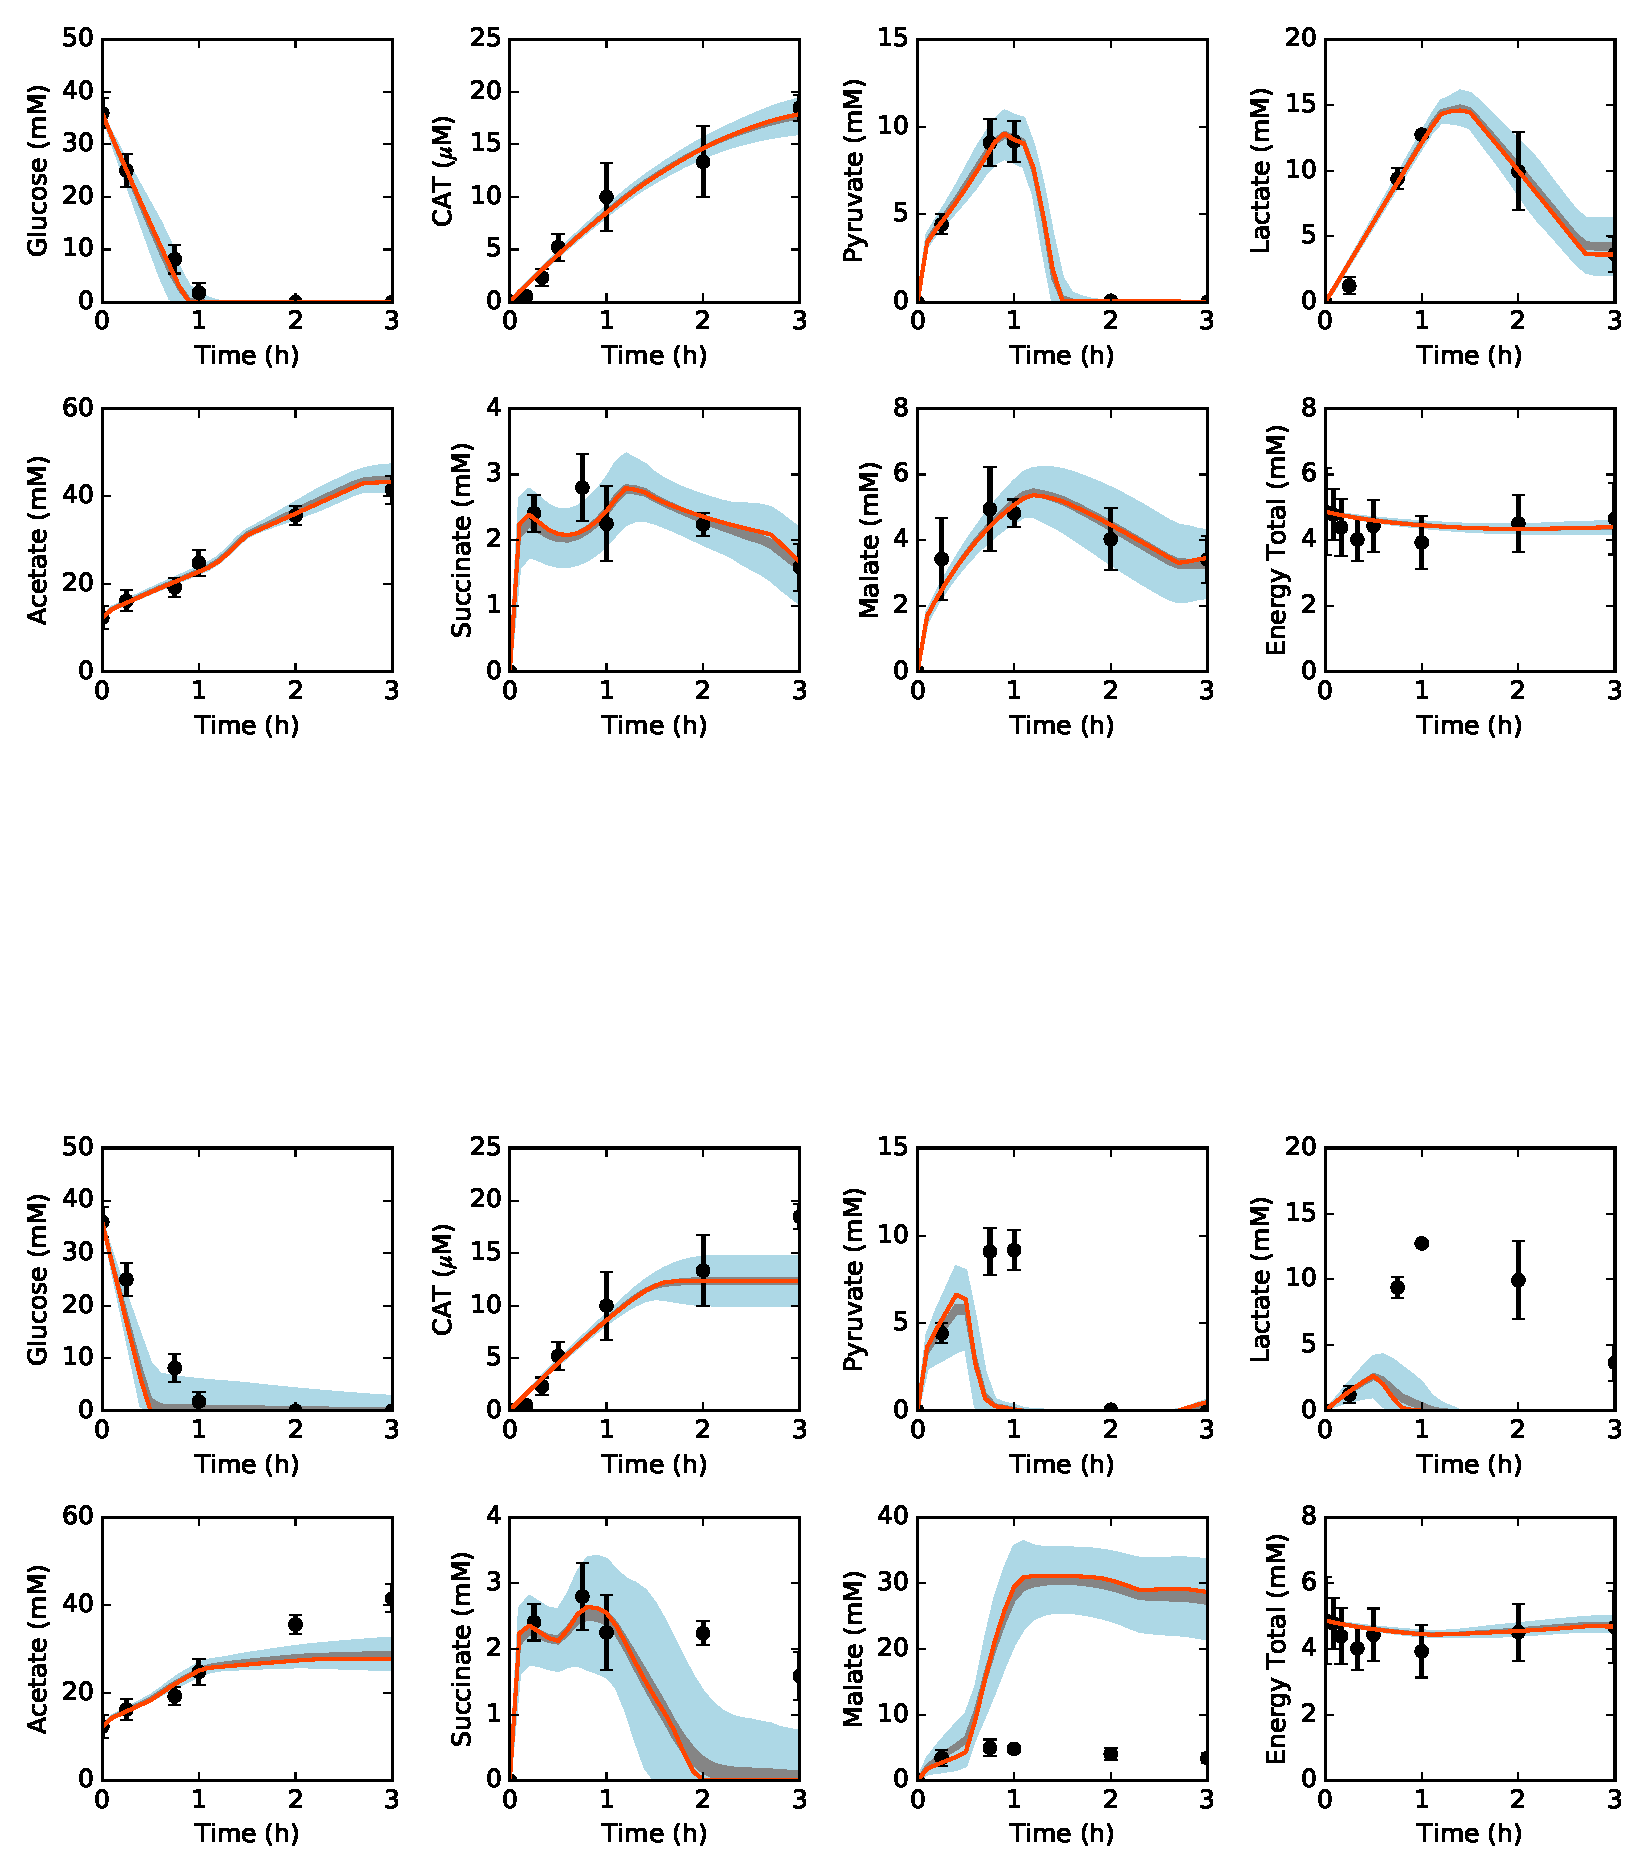
\includegraphics[width=1.00\textwidth]{./Figures/CarbonBoth.pdf}
% \caption{Central carbon metabolism in the presence (top) and absence (bottom) of allosteric control, including glucose (substrate), CAT (product), and intermediates, as well as total concentration of energy species. Best-fit parameter set (orange line) versus experimental data (points). 95\% confidence interval (blue shaded region) and 95\% confidence interval of the mean (gray shaded region) over the ensemble of 100 sets.}
% \label{fig:CarbonBoth}
% \end{figure}

\begin{figure}[ht]
\centering
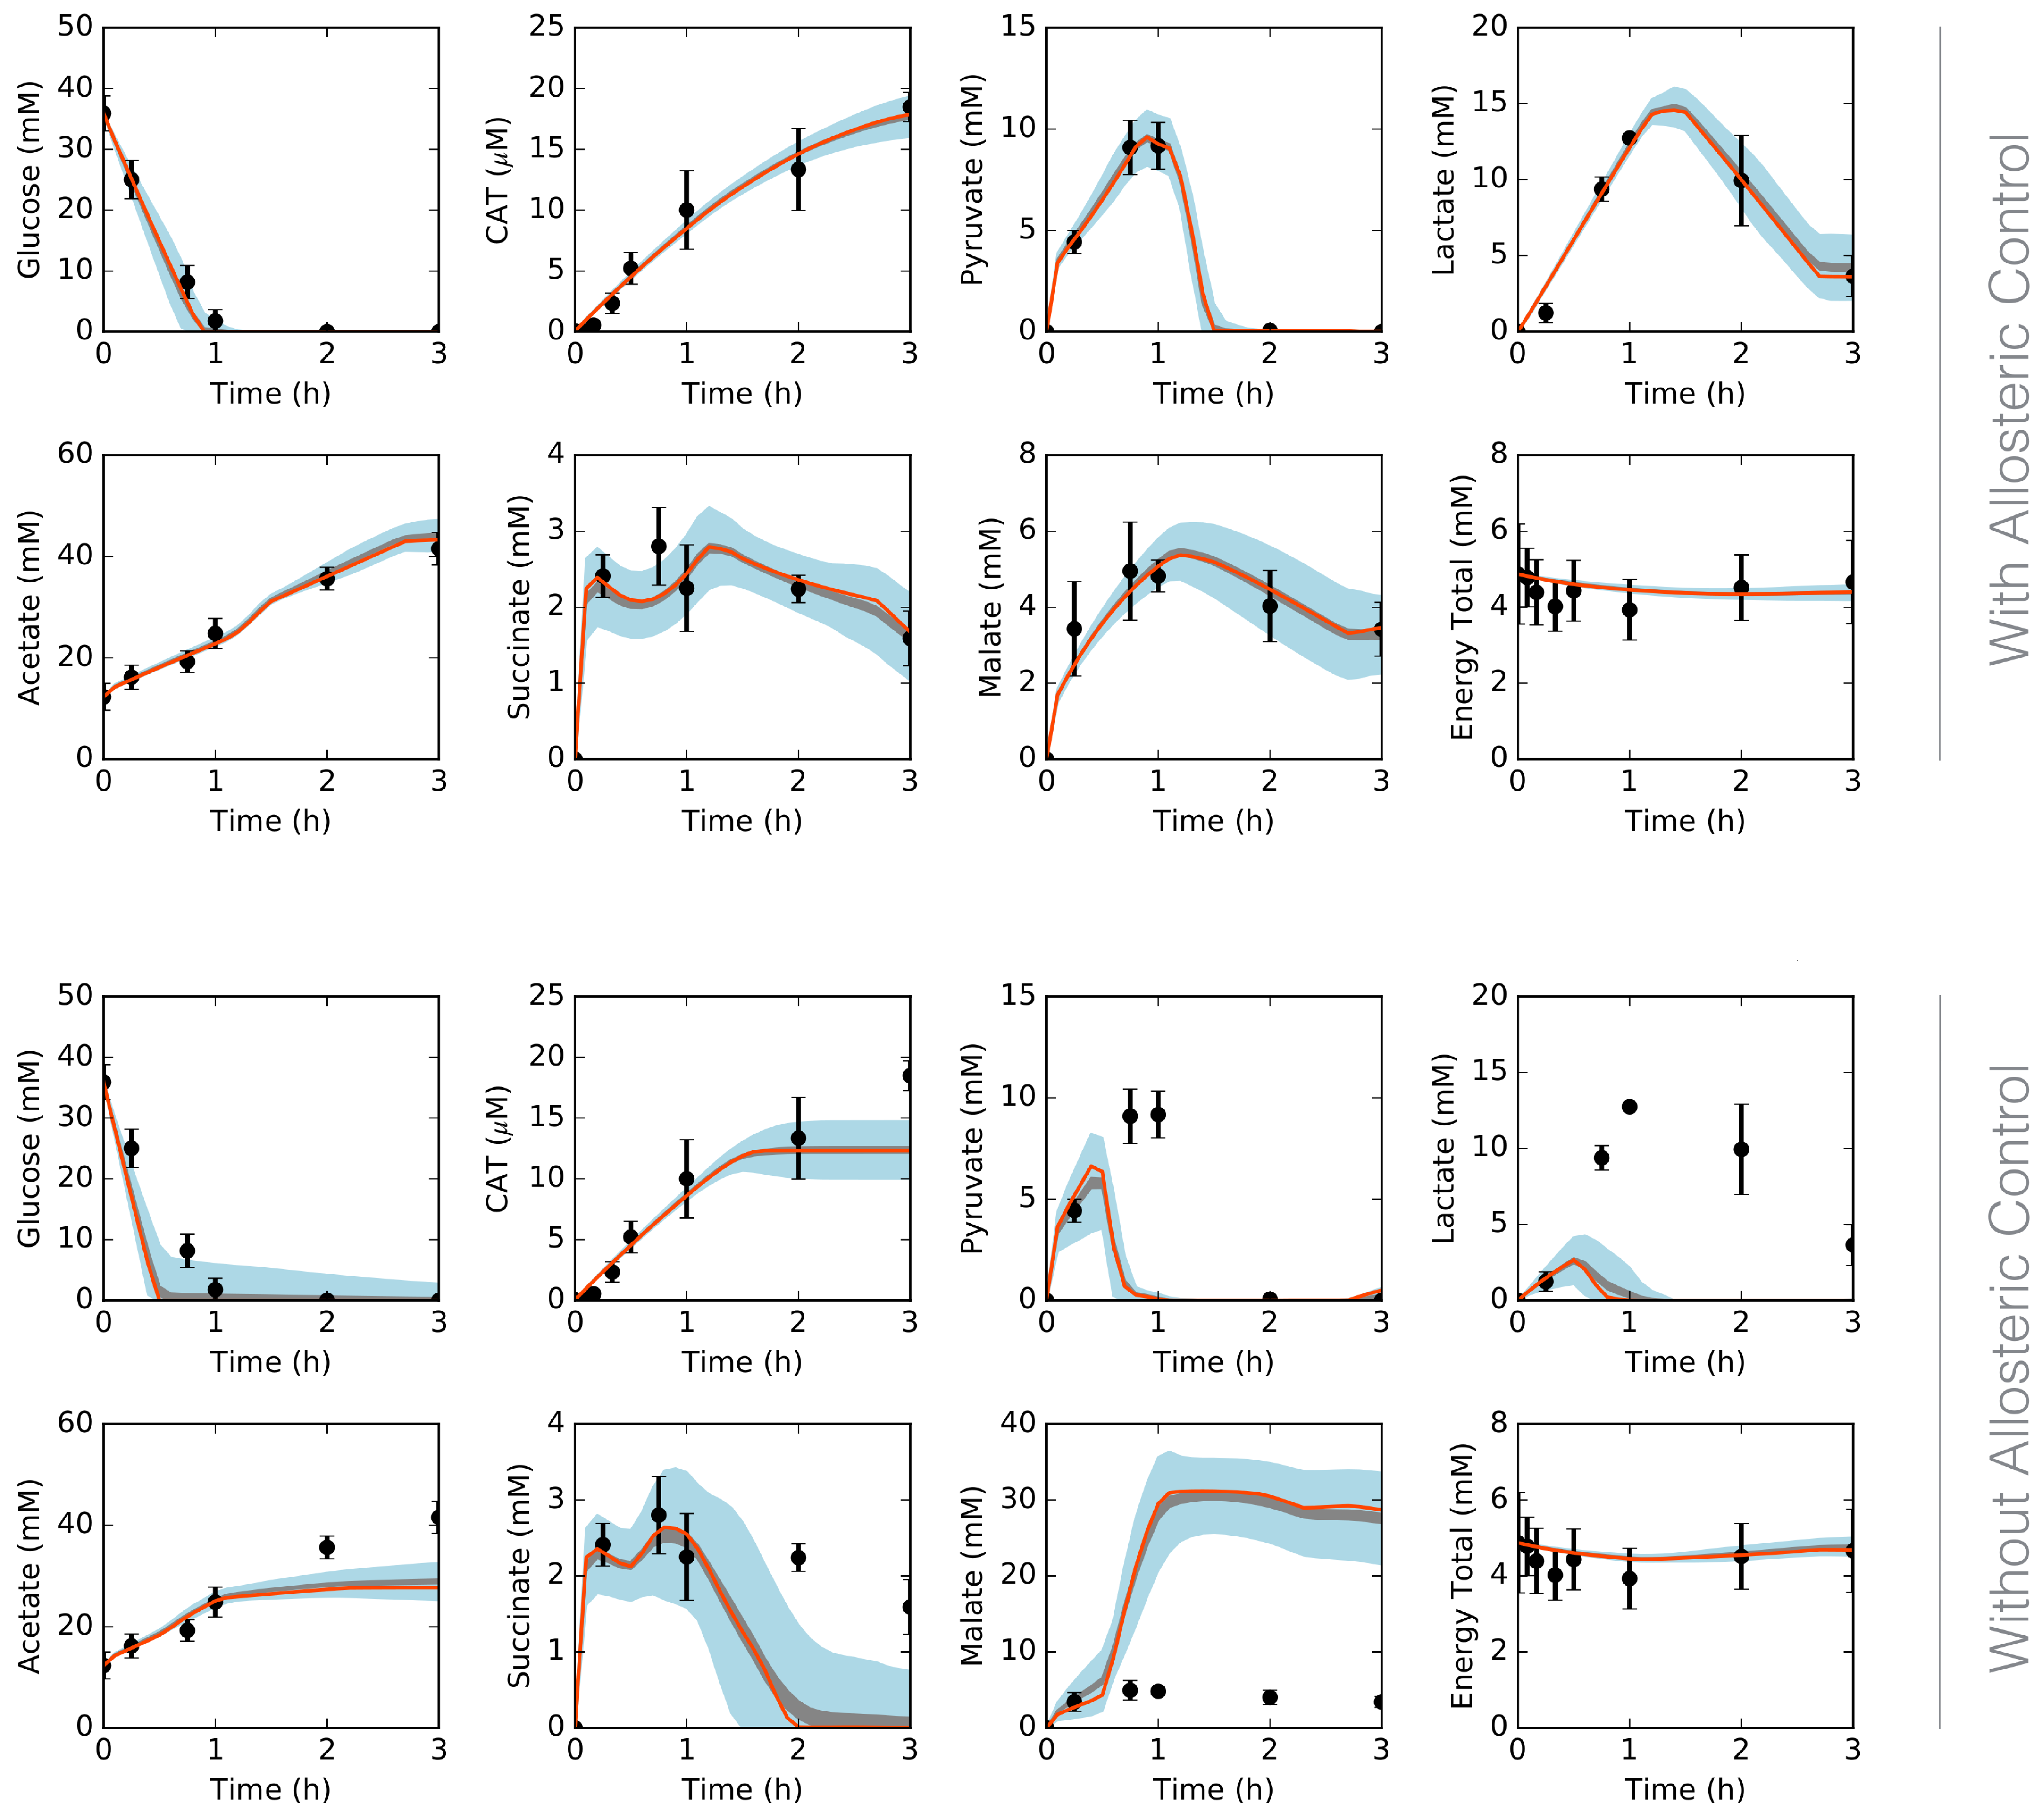
\includegraphics[width=1.00\textwidth]{./Figures/CarbonBoth_png.pdf}
\caption{Central carbon metabolism in the presence (top) and absence (bottom) of allosteric control, including glucose (substrate), CAT (product), and intermediates, as well as total concentration of energy species. Best-fit parameter set (orange line) versus experimental data (points). 95\% confidence interval (blue shaded region) and 95\% confidence interval of the mean (gray shaded region) over the ensemble of 100 sets.}
\label{fig:CarbonBoth}
\end{figure}

\begin{figure}[ht]
\centering
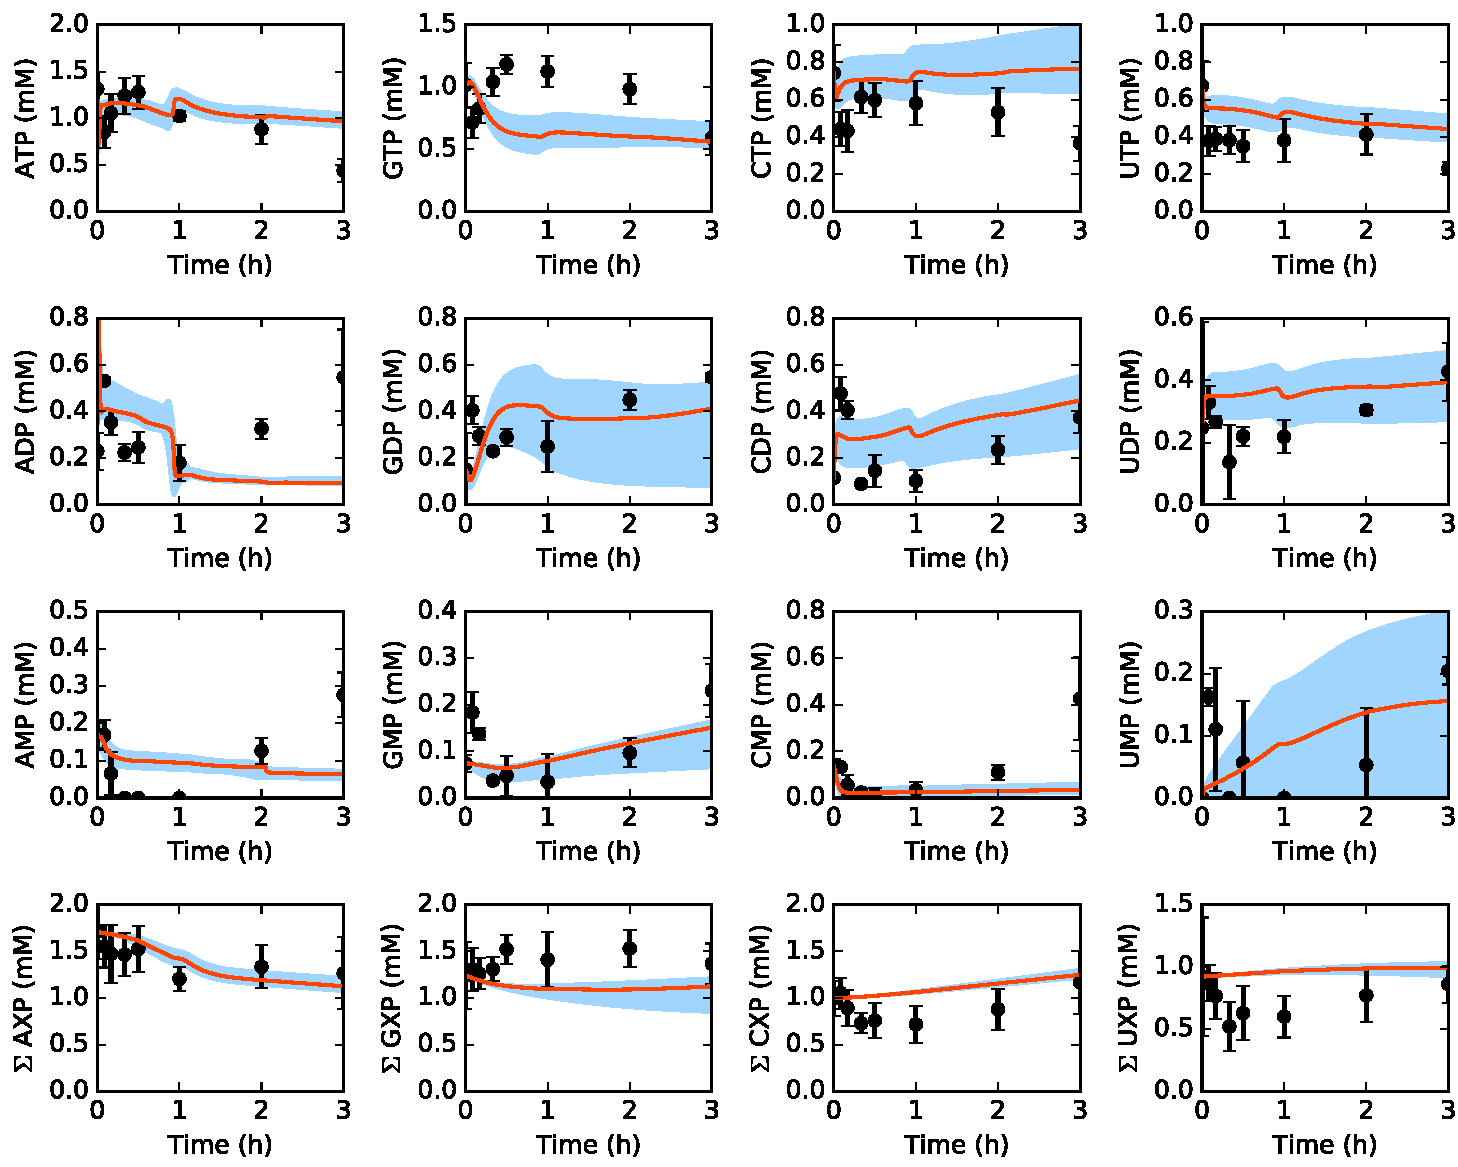
\includegraphics[width=1.00\textwidth]{./Figures/Energy.pdf}
\caption{Energy species and energy totals by base in the presence of allosteric control. Best-fit parameter set (orange line) versus experimental data (points). 95\% confidence interval (blue shaded region) and 95\% confidence interval of the mean (gray shaded region) over the ensemble of 100 sets.}
\label{fig:Energy}
\end{figure}

\begin{figure}[ht]
\centering
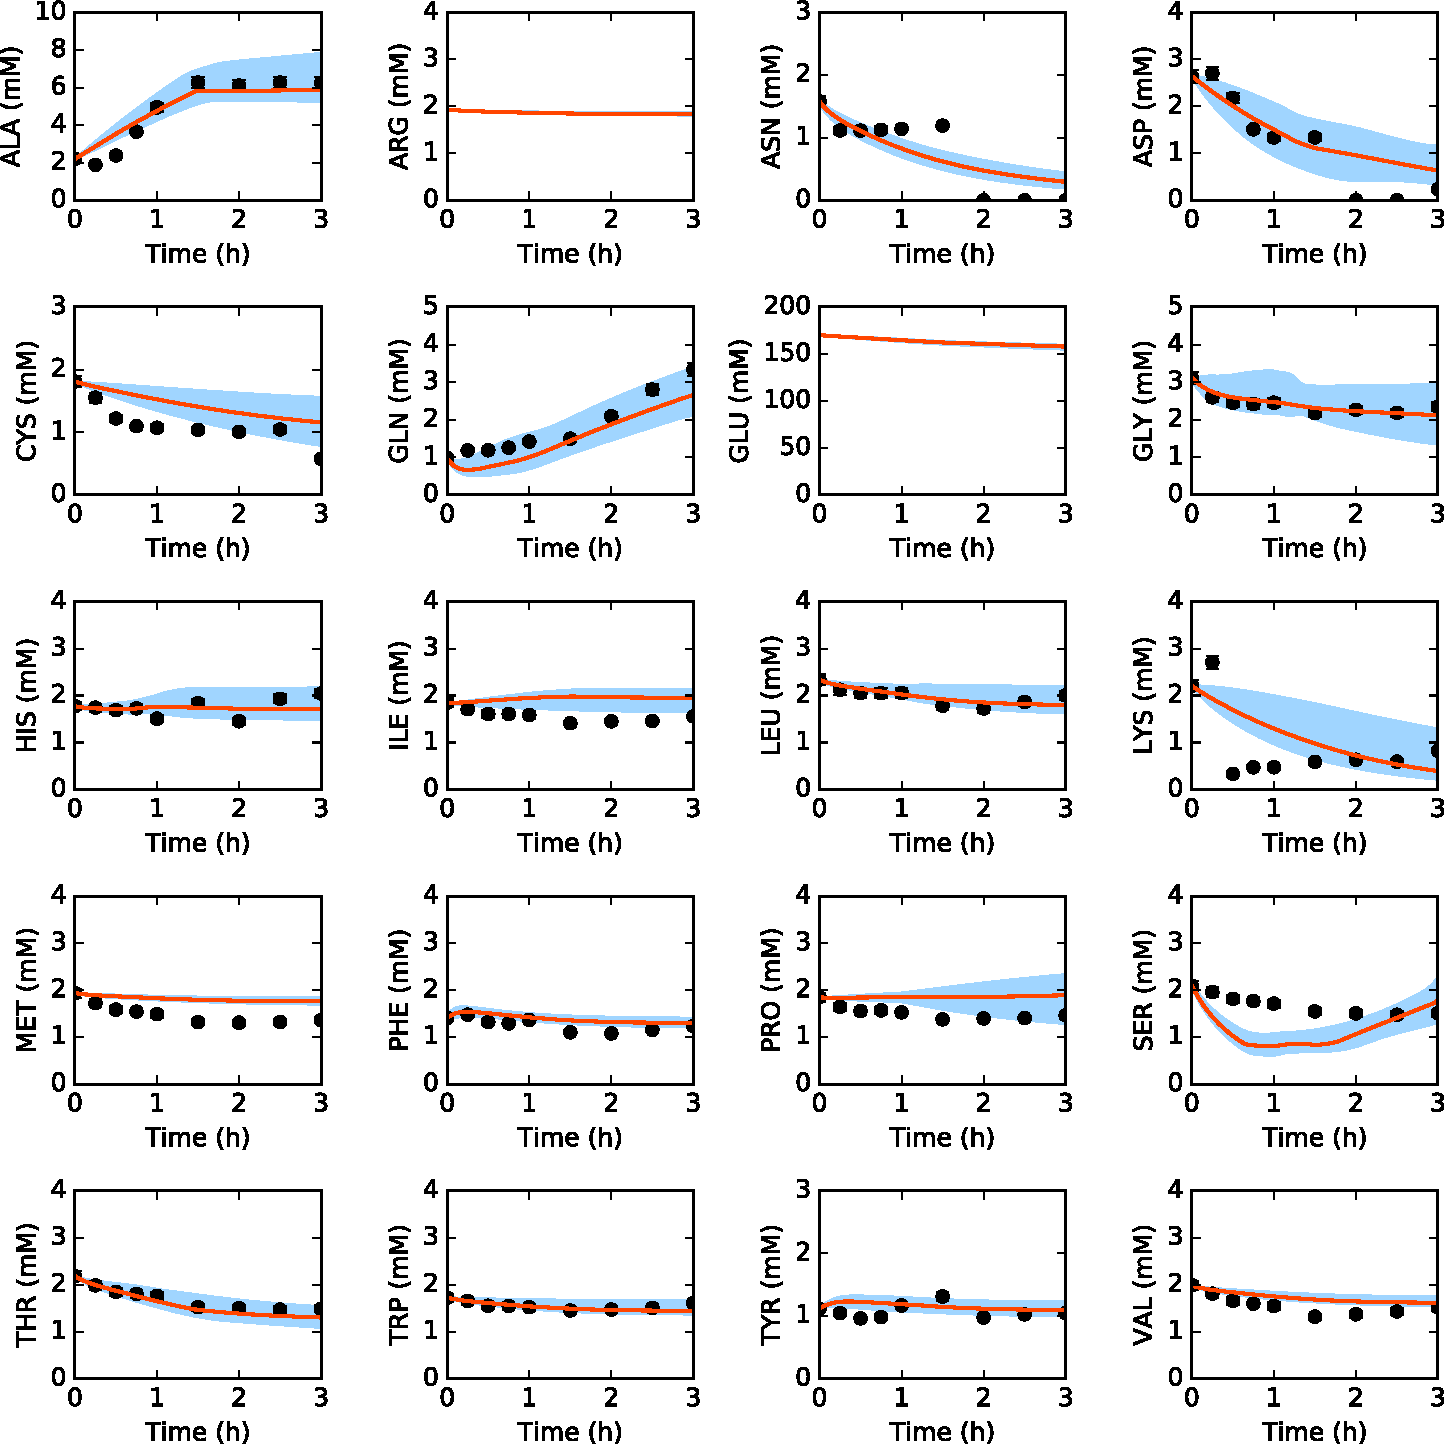
\includegraphics[width=1.00\textwidth]{./Figures/Amino.pdf}
\caption{Amino acids in the presence of allosteric control. Best-fit parameter set (orange line) versus experimental data (points). 95\% confidence interval (blue shaded region) and 95\% confidence interval of the mean (gray shaded region) over the ensemble of 100 sets.}
\label{fig:Amino}
\end{figure}

\begin{figure}[ht]
\centering
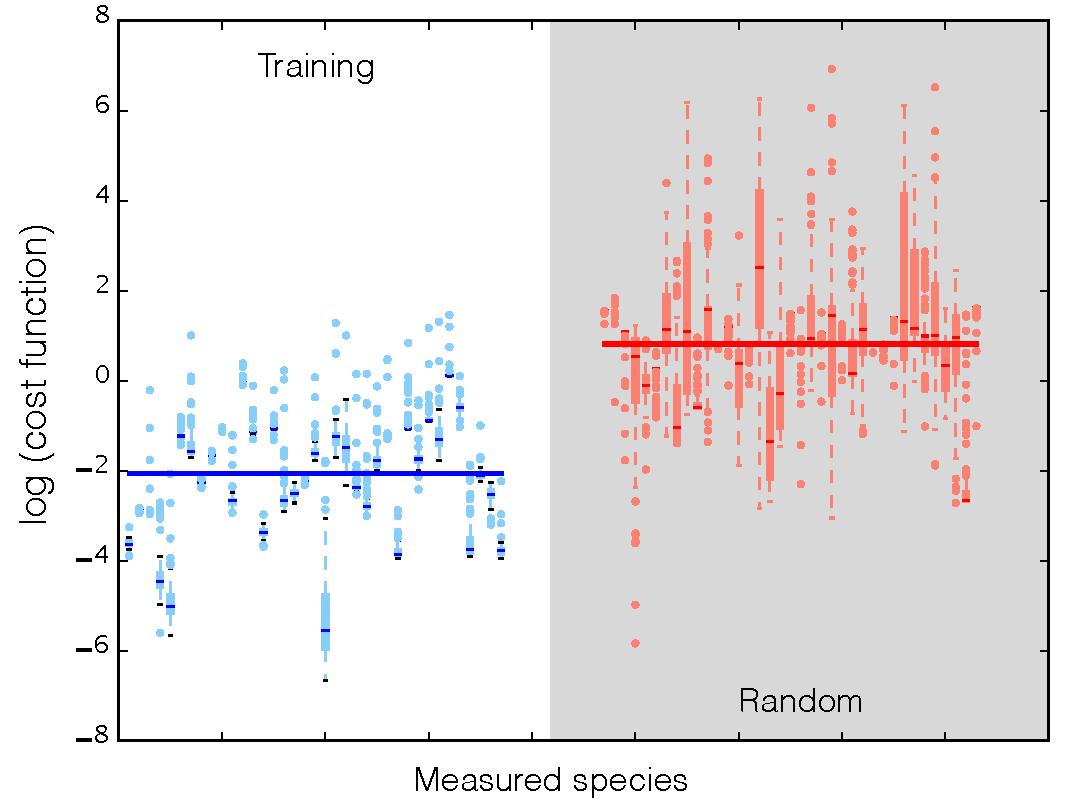
\includegraphics[width=1.00\textwidth]{./Figures/BoxPlot-KCFM.pdf}
\caption{Log of cost function across 37 datasets for data-trained ensemble (blue) and randomly generated ensemble (red, gray background). Median (bars), interquartile range (boxes), range excluding outliers (dashed lines), and outliers (circles) for each dataset. Median across all datasets (large bar overlaid).}
\label{fig:BoxPlot}
\end{figure}

\begin{figure}[ht]
\centering
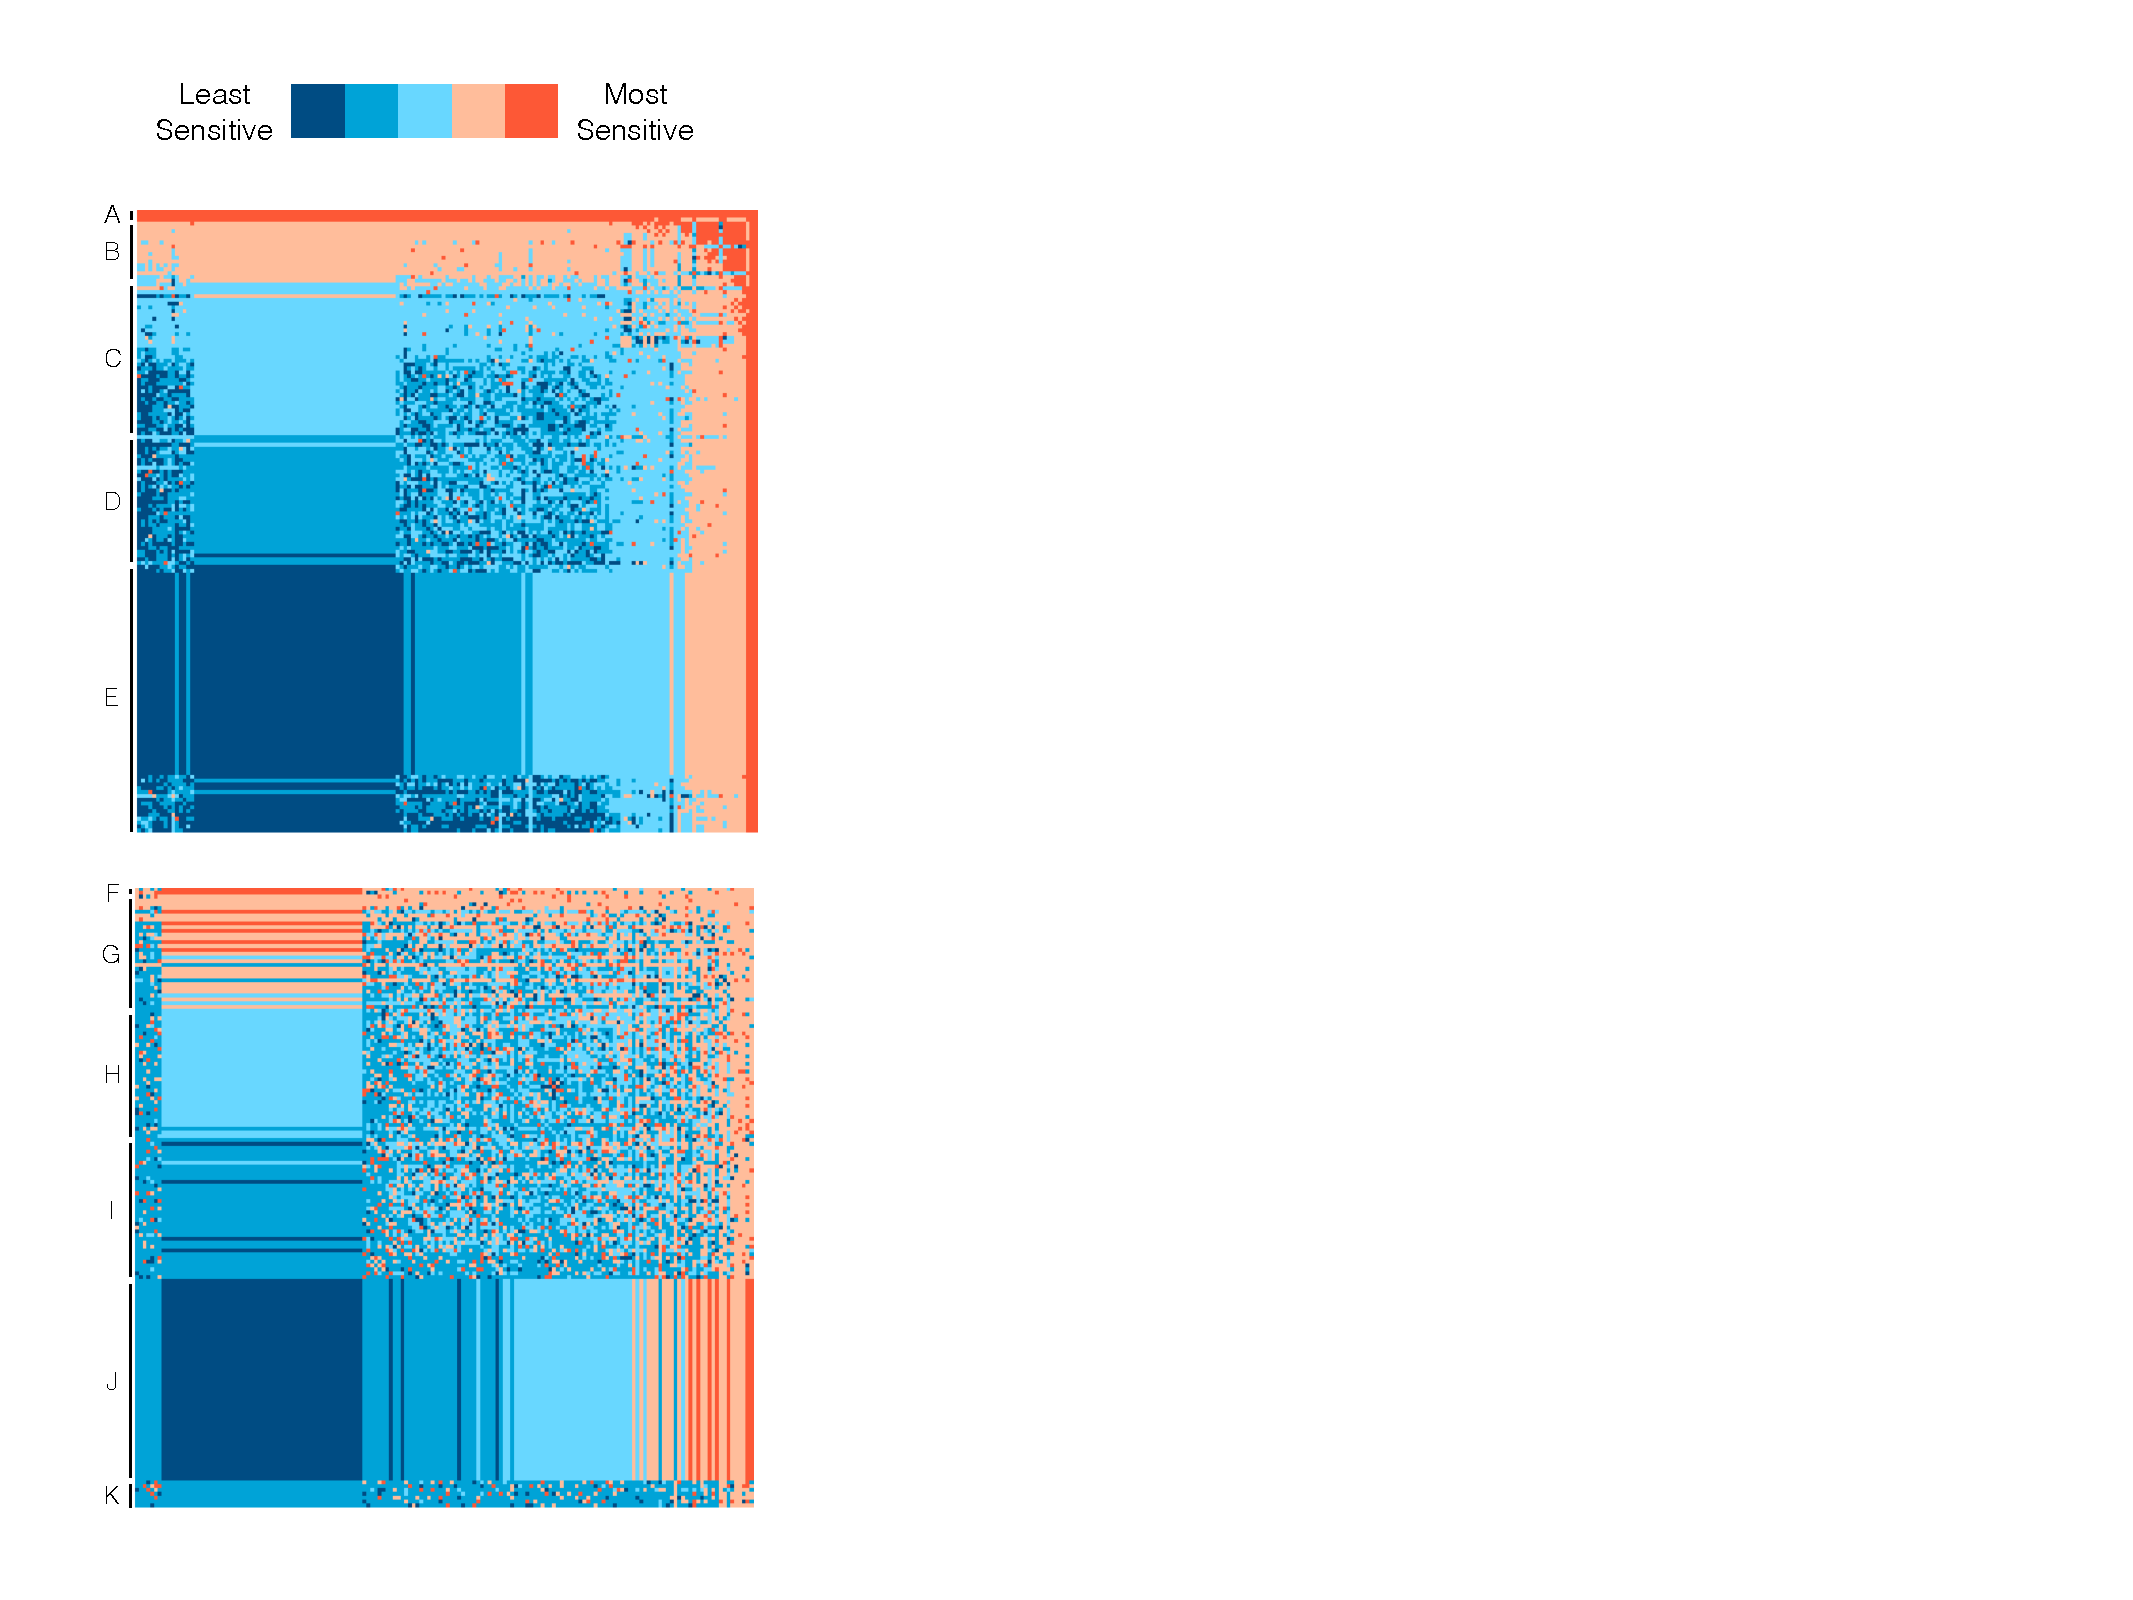
\includegraphics[width=0.76\textwidth,trim=0 28 615 40,clip]{./Figures/Sensitivity.pdf}
\caption{Normalized first-order and pairwise sensitivities of CAT production (top) and system state (bottom) to rate constants.}
\label{fig:Sensitivity}
\end{figure}

\begin{figure}[ht]
\centering
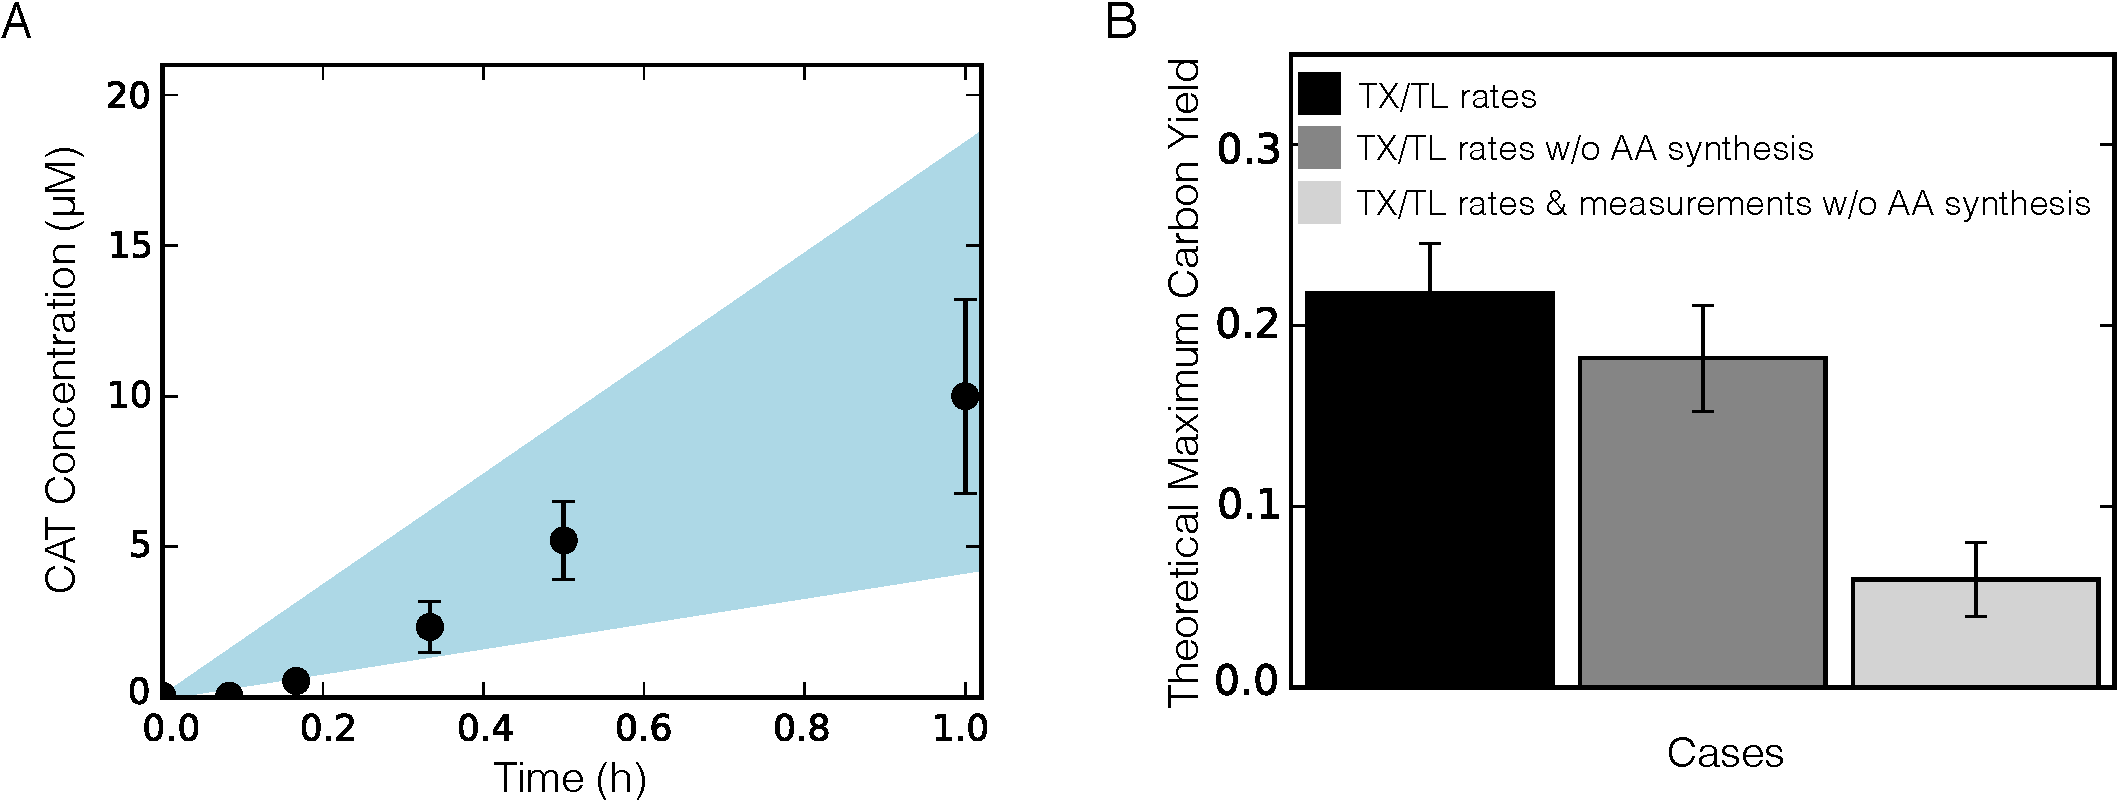
\includegraphics[width=0.95\textwidth]{./Figures/CAT_prod_yield.pdf}
\caption{Sequence-specific flux balance analysis of CAT production and yield. A. 95\% confidence interval of the ensemble (light blue region) for CAT concentration versus time. B. Theoretical maximum carbon yield of CAT calcualted by ssFBA for three different cases: unconstrained except for glucose uptake (black), constrained by transcription/translation (TX/TL) rates (grey), and constrained by transcription/translation (TX/TL) rates and experimental measurements where available (light grey). Error bars represent standard deviation of the ensemble.}
\label{fig:CATProdYield}
\end{figure}

\begin{figure}[ht]
\centering
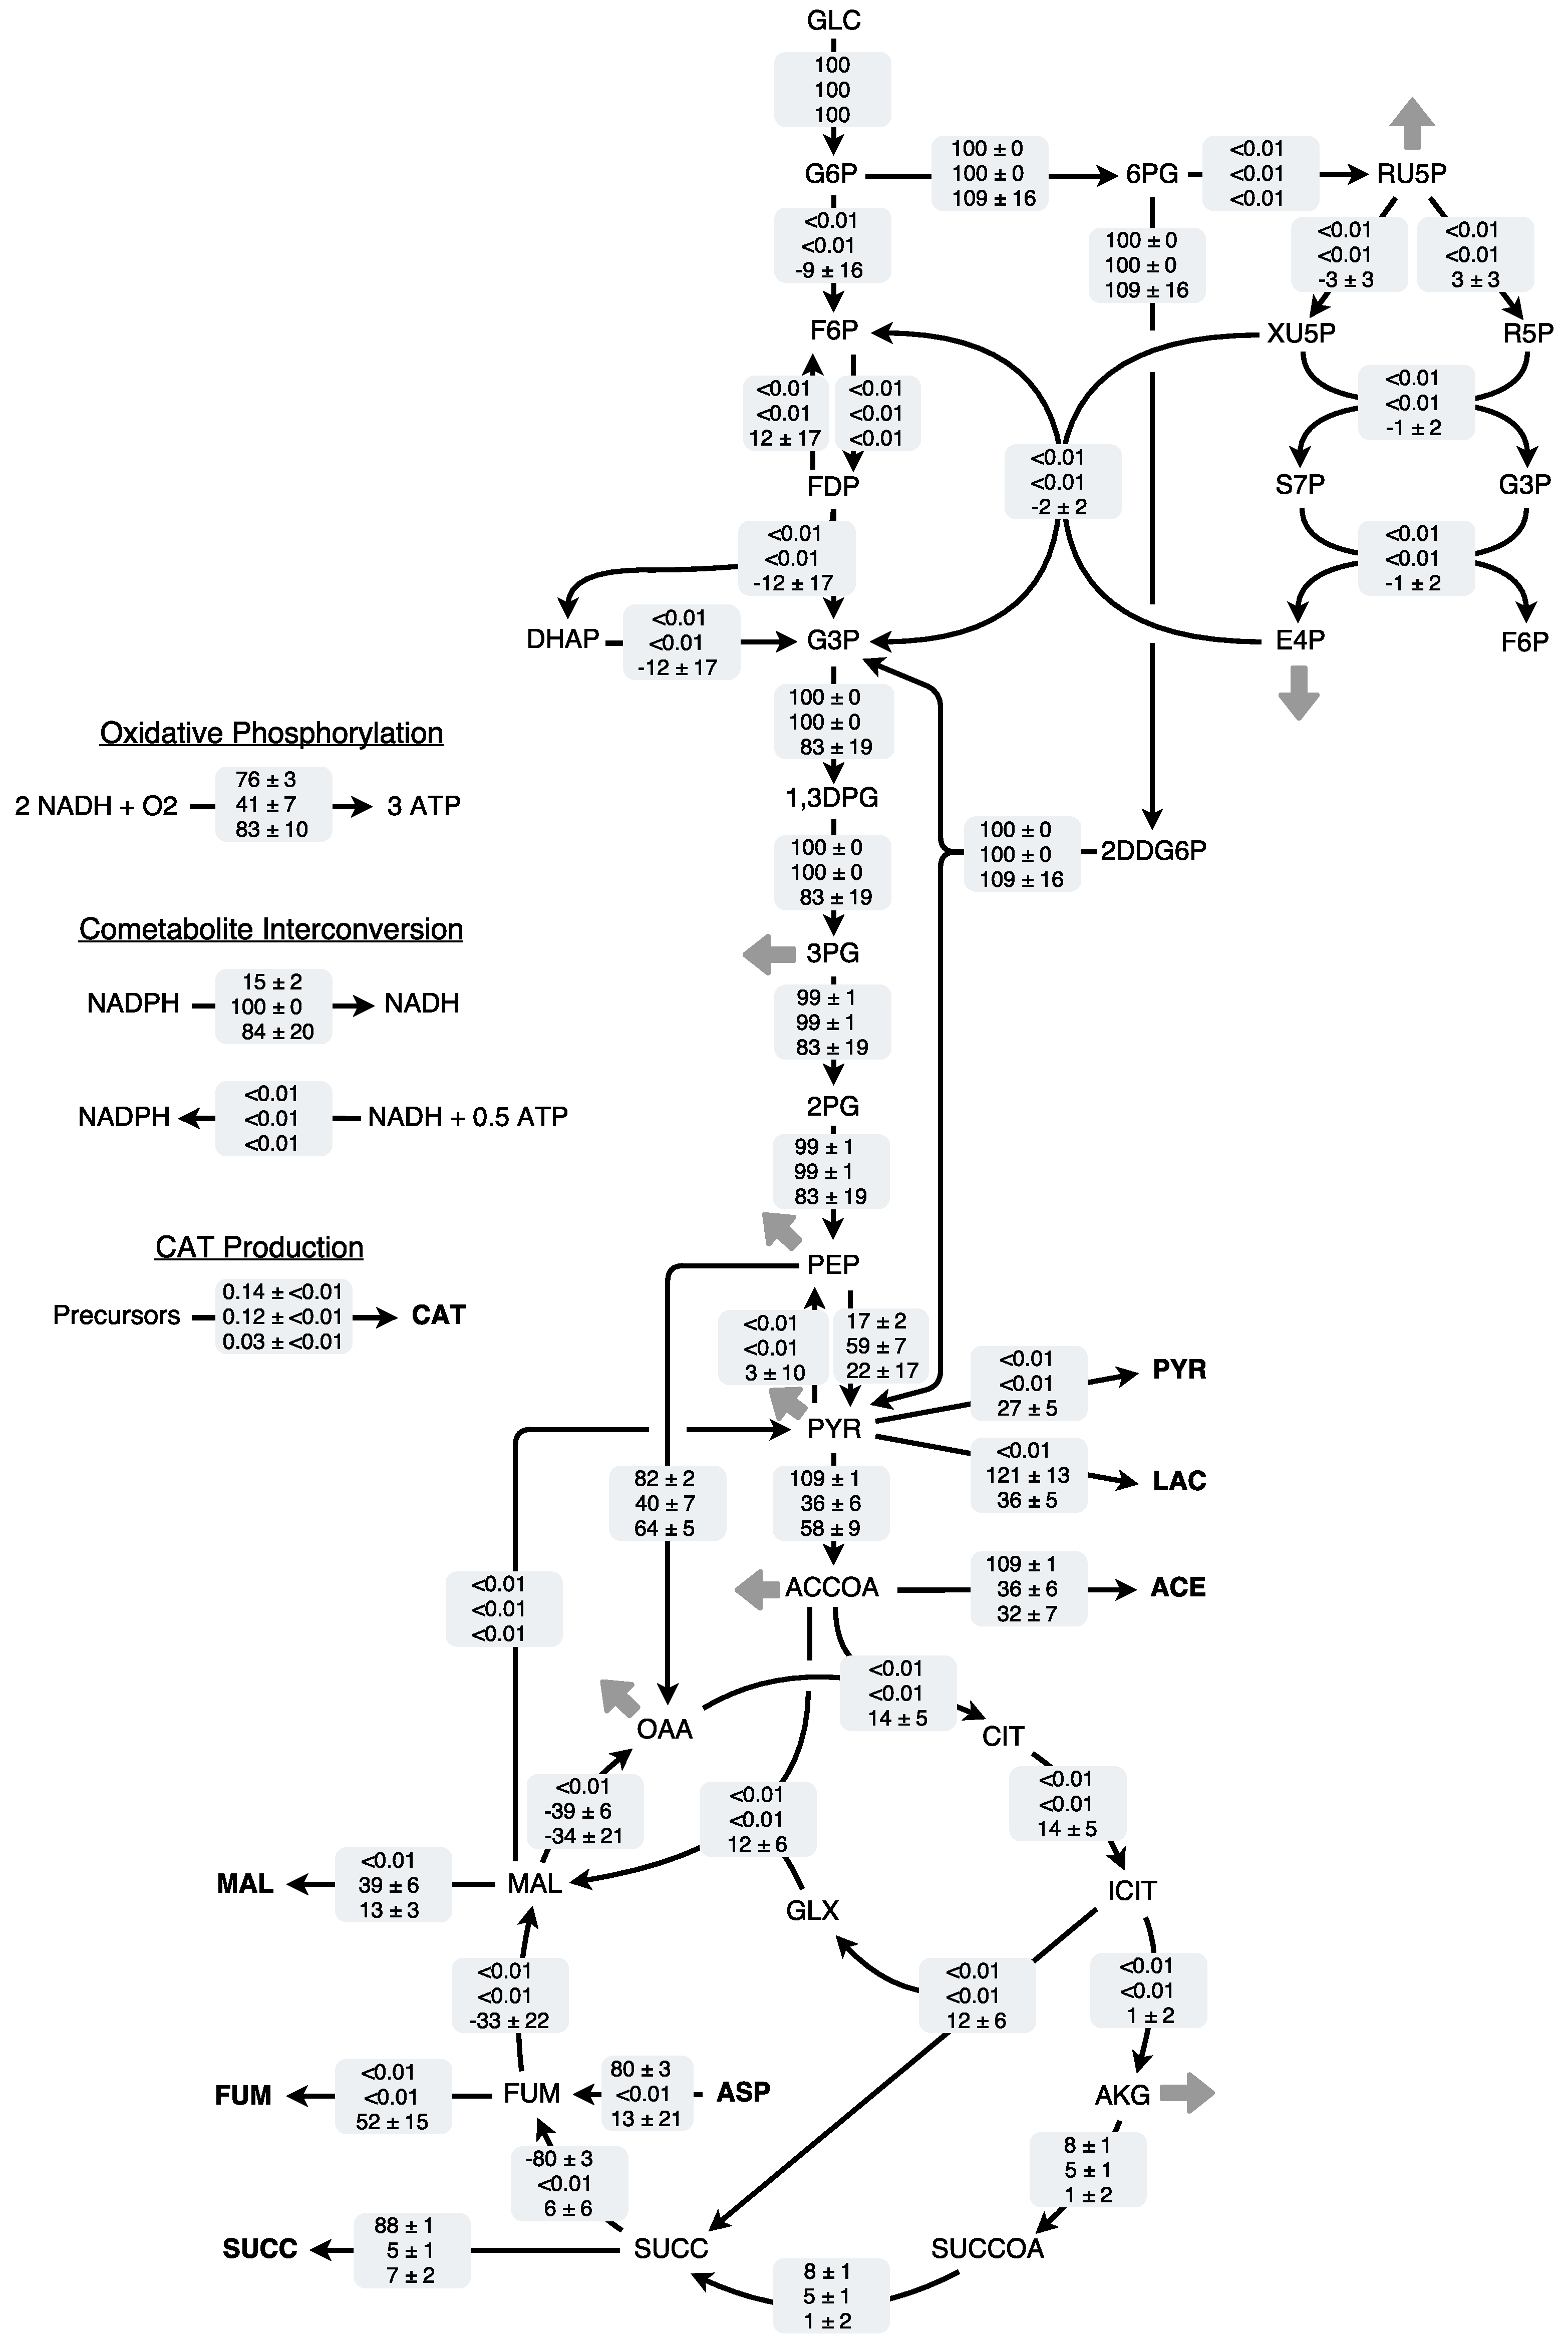
\includegraphics[width=0.8\textwidth]{./Figures/CAT_flux_final.pdf}
\caption{Flux profile for glycolysis, pentose phosphate pathway, Entner-Doudoroff pathway, TCA cycle, NADPH/NADH transfer, and oxidative phosphorylation. Sequence-specific FBA flux value (mean ± standard deviation) across ensemble for 1 hr, normalized to glucose uptake flux. Flux distribution for three different cases: unconstrained except for glucose uptake (top row), constrained by transcription and translation rates (second row), and constrained by transcription, translation rates and experimental measurements where available (bottom row).}
\label{fig:Network}
\end{figure}

\clearpage

% Supplemental figures -
% Set the S-
\renewcommand\thefigure{S\arabic{figure}}
\renewcommand\thetable{T\arabic{table}}
\renewcommand\thepage{S-\arabic{page}}
\renewcommand\theequation{S\arabic{equation}}

% Reset the counters -
\setcounter{equation}{0}
\setcounter{table}{0}
\setcounter{figure}{0}
\setcounter{page}{1}

% Supplemental figures go here ...
%\begin{figure}[ht]
%\centering
%\includegraphics[width=1.00\textwidth]{./figs/<Filename>.pdf}
%\caption{Captiontext goes here}
%}\label{fig:<label_name>}
%\end{figure}

\end{document}
\grid
\grid
